\documentclass[11pt,a4paper,twoside]{report}
\usepackage{graphicx}
\usepackage{graphics}
\usepackage{tabularx}
\usepackage{listings}
\usepackage{color}
\usepackage{layout}
\usepackage{fancyhdr}
\usepackage{amsmath}
\usepackage{syntax}

%\setlength{\marginparwidth}{24pt}
\setlength{\textwidth}{390pt}
\setlength{\grammarindent}{12em}
\setlength{\grammarparsep}{20pt plus 1pt minus 1pt}
\setlength{\oddsidemargin}{42pt}
\setlength{\evensidemargin}{30pt}


\definecolor{dkgreen}{rgb}{0,0.6,0}
\definecolor{gray}{rgb}{0.5,0.5,0.5}
\definecolor{mauve}{rgb}{0.58,0,0.82}

\lstset{
  basicstyle=\footnotesize,    % the size of the fonts that are used for the code
  numbers=left,                % where to put the line-numbers
  numberstyle=\footnotesize,   % the size of the fonts  for the line-numbers
  stepnumber=1,
  numbersep=1pt,               % how far the line-numbers are from the code
  backgroundcolor=\color{white},    
  showspaces=false,            % show spaces adding particular underscores
  showstringspaces=false,      % underline spaces within strings
  showtabs=false,              % show tabs within strings
  frame=trb,                % adds a frame around the code
  tabsize=2,                   % sets default tabsize to 2 spaces
  captionpos=b,                % sets the caption-position to bottom
  breaklines=true,             % sets automatic line breaking
  breakatwhitespace=false,   
  keywordstyle=\color{blue},        % keyword style
  commentstyle=\color{dkgreen},     % comment style
  stringstyle=\color{mauve}
}


\pagestyle{fancy}
\fancyhf{}
\lhead{\nouppercase{\leftmark}}
\rhead{\nouppercase{\rightmark}}
\fancyfoot[C]{\thepage}


\begin{document}
\begin{titlepage}
\thispagestyle{empty}

%\fancyhf{}
\begin{center}
\Large{Imperial College of Science, Technology and Medicine}\\
\Large{Department of Computing}\\[5.0cm]

\Huge{\textbf{Dron: An Integration Job Scheduler}}\\[1.0cm]
\Huge{Ionel Corneliu Gog}\\[0.5cm]
\normalsize{Supervisor: Peter Pietzuch}\\
\normalsize{Second Marker: Alastair Donaldson}\\[8.0cm]

\normalsize{Submitted in part fulfilment of the requirements for the}\\
\normalsize{MEng Honours degree in Computing of Imperial College, June 2012}
\end{center}
\end{titlepage}

\newpage
\thispagestyle{empty}
\mbox{}
\newpage
\thispagestyle{plain}
\begin{center}
\large{\textbf{Abstract}}
\end{center}
\normalsize{}
\vspace{1.5cm}
\noindent
Data analysis has become a key aspect of many companies day to day activities. Systems have been develop to run large data computations on thousands of machines. Moreover, on top of this infracture many higher level frameworks have been deployed. Despite the plethora of systems, no current scheduler has been built to encourage execution of multi-framework workflows.\\

\noindent
In this report we describe Dron, a new job scheduler that makes it easy to use multiple frameworks. On one hand, it allows engineers to easily integrate frameworks to work with the scheduler, and on the other hand, it provides a language for users to create job workflows. We will then show that Dron scales better than other currently available workflow schedulers. Following, we also study four scheduling strategies that utilize the graph of job dependencies in order to optimize resource utilization. Lastly, we demonstrate the powerfulness of the system by using it to build a recommendation engine.


\newpage
\thispagestyle{empty}
\mbox{}
\newpage
\thispagestyle{plain}
\begin{center}
\large{\textbf{Acknowledgements}}
\end{center}
\normalsize{}

\vspace{1.5cm}
\noindent
First and foremost, I would like to thank to my mother Maria and to my sister Antonia. Without their support I would have not been able to pursue my dreams and to be the person I am today.\\

\noindent
Secondly, I would like to thank to Peter Pietzuch and Alastair Donaldson for the advices they have given me through the the course of the project.\\

\noindent
Finally, I would also like to thank to Delia David for the information she has given me about the systems deployed at Facebook.

\newpage
\thispagestyle{empty}
\mbox{}
\newpage
\tableofcontents
\newpage

\chapter{Introduction}
\section{Motivation}
The amount of digital information is growing at an astonishing pace. A study conducted by Gantz and Reinsel~\cite{IDC} correctly predicted that the quantity of data created on the Internet in 2011 would exceed 1.8 zettabytes. Every month we created more data than the entire size of the Internet up to 2007.


The exponential increase of stored information has made data analysis a key research topic. The interest was also sustained by the need of many Internet companies to analyze the collected data sets in order to improve their products and sustain innovation. Thus, the increase in stored data has come to be a nuisance for some people. Traditional Relational Database Management Systems (RDBMS) can not scale up to meet the requirements. Even with all the advances in hard drives and multi-core programming, the fastest machines can not support the intensive data processing.


The high costs of buying specially designed servers together with the above mentioned reasons, have encouraged Google, followed by many other companies, to develop an infrastructure based on commodity hardware. However, the new type of clusters also have many drawbacks. For example, in a typical first year, in a new Google cluster, approximatively 5 racks misbehave causing up to 50\% package loss, 20 racks fail making 40 to 80 machines dissappear for up to 6 hours. This has brought fault tolerance to the core of infrastructure development, and as a result an abundance of scalable, failure tolerant computing frameworks have been developed (e.g. MapReduce~\cite{MapReduce}, Hadoop~\cite{Hadoop}, Dryad~\cite{Dryad,DryadLinq}).


Given that the aforementioned systems were built for software engineers, they do not provide the abstractions needed by the layman users. Thus, more and more tools have been developed on top of the frameworks. Their purpose is to cover a new variety of use cases and to simplify usage.


Facebook has developed Hive~\cite{Hive} so that engineers can run SQL like queries on their 100+ Petabyte Hadoop cluster, Yahoo has developed Pig Latin~\cite{Pig} a combination of SQL queries and MapReduce style procedural programming. Moreover, Google has built many tools like Sawzall~\cite{Sawzall} and FlumeJava~\cite{FlumeJava} around its MapReduce framework in order to conduct log analysis, store old data and perform graph algorithms as a series of chained MapReduce jobs.


With the abundance of frameworks and tools developed for specific tasks, engineers have started to create workflows that make use of multiple systems. As presented in~\cite{FacebookWarehouse}, Facebook uses an entire suite of systems in order to conduct data analysis. For example, Scribe~\cite{Scribe} is used to move data from their web tiers to HDFS~\cite{HDFS}. Moreover, jobs that scrape the federated MySQL databases, containing all website related data, are run on daily basis. Lastly, data is transformed into Hive readable format and log analysis is conducted. However, since the amount of data copied varies from hour to hour, data analysts do not have an easy way to manage their workflows and to conduct experiments.


In this report we will describe a new system called Dron, that will attempt to close the above described gap. The purpose of Dron is to make frameworks more interoperable by providing an integration job scheduler that can handle job dependencies. The scheduler will allow users to define large workflows that make use of multiple systems. It will display information about data and jobs so that similar steps within different workflows will be identified and performed only once.

\section{Contributions}
This project made the following contributions:
\begin{itemize}
\item{}
\textbf{Developed New Job Scheduler}\\
We developed a highly scalable and fault tolerant job scheduler that is able to handle thousands of jobs a second, distributed over many machines. The jobs are Unix commands (e.g. copy, Hadoop command, Hive query) that are required to be executed only once or at given time intervals. They can also depend on the execution of other jobs which means that they are only run if all their dependencies have been successfully executed.
\item{}
\textbf{Integration of Multiple Frameworks}\\
We demonstrated the ease of adapting current infrastructure systems to cooperate with Dron for job scheduling. We modified three framworks (Hadoop, Mahout and Spark) to show how to use the API we have provided.
\item{}
\textbf{Removed Duplicated Computation Within a Data Center}\\
By placing Dron at the core of every job computation, we allowed it to capture the entire graph of job and resource dependencies. Thus, by consulting the graph, users can avoid conducting the same computation more than once.
\item{}
\textbf{Evaluated Several Scheduling Strategies}\\
We have built a benchmark modelled after real world computations. We have also studied four scheduling strategies that use the direct acyclic graph of job dependencies in order to reduce the running time of the benchmark.
\item{}
\textbf{Opened Opportunities for New Systems}\\
By bringing the state of the art frameworks together, in a data center, and by providing a way of creating complex workflows, we allow for new computations and systems (e.g. a recommendation engine) to be expressed as a series of Dron jobs.
\item{}
\textbf{Developed and Evaluated Two System Architectures}\\
We have implemented two versions of Dron and we have discussed their advantages and disadvantages.
\item{}
\textbf{Fault Tolerant Implementation}\\
We have implemented a system that offers a good degree of fault tolerance. Moreover, we have discussed the behaviour of the system under different failure scenarios.
\item{}
\textbf{Scalability Evaluation}\\
We evaluated the scalability of Dron by performing a variety of tests whose aim was to measure the behaviour of the system under different types of load. The benchmarks tested how the schedulling delay is affected when the number of jobs increases and how many concurrent running jobs the system can handle at a time. Finally, We also compared Dron with the current state of the art workflow manager.
\end{itemize}

\section{Outline of this report}
We continue with Chapter 2 where we provide an overview of the current existing solutions for running large process or data intensive computations. While presenting each framework we also briefly discuss its use cases. The second part of the chapter is devoted to other state of the art workflow job schedulers which may have few similarities with our system.


Following, in Chapter 3 we give an overview of the highly scalable and fault tolerant system we developed to tackle the existing problems. We do so by first describing the features of the system, the API it provides and its dependency language. Following, we give a high overview of its architecture. Lastly, we focus on the several implementation iterations we conducted and explain the rationale behind our current system design. The optimizations and issues encountered while developing the system are also discussed.


Chapter 4 demonstrates the easiness of adapting frameworks to work with the new job scheduler. First, we go over the possibilities of integration provided by Dron. Subsequently, we exemplify the changes we had to make to each system.


In Chapter 5 we evaluate the performance of Dron by conducting several tests that stress its ability to handle a large volume of different jobs. Moreover, we also use a benchmark designed after the jobs Facebook is running to analyse the system's suitability for current industry needs. Using the benchmark we also evaluate four scheduling strategies that make use of the dependencies graph. Following we compare Dron with Oozie, the most used workflow scheduler. Lastly, we discuss Dron's fault tolerance under different situations.


Chapter 6 exemplifies the opportunity of building new systems on top of the job scheduler. We show the development of a recommendation engine using Dron and several of the frameworks we adapted.


Lastly, in Conclusions (Chapter 7) we provide a retrospective of the project, analyse if we have reached our goals, mention the lessons we learned and outline the areas for future work.

\chapter{Background}
Workflow scheduling and management has been a perpetual research topic since the invention of the first batch computer, up to grid computing and distributed software frameworks. Even tough, much research has been conducted in the area we believe that there still are plenty of opportunities once with the development of the new large cluster computation frameworks.


In the first few sections of the chapter we will briefly explain how several current frameworks work. They will help us understand how large data analysis is conducted, and why there is a genuinely need for a new framework management system. Moreover, the first few sections will give us the background required to analyze current state of the art alternatives to Dron.

\section{MapReduce}
\label{sec:MapReduce}
The concepts behind MapReduce were introduced in a paper by Dean and Ghemawat~\cite{MapReduce}. It is a \textit{programming model} associated with a highly scalable framework for computation on large data sets. As the authors acknowledged, the abstractions behind MapReduce were inspired by the map and reduce primitives present in Lisp and many other functional programming languages.


A MapReduce job receives as input a set of key/value pairs and returns as output a possibly different set of pairs. The framework does not restrict the types of the input and output. Users can pass to a job from simple pairs of integers up to complex files location.


MapReduce conducts the processing with the help of two functions provided by the users: \textit{Map} and \textit{Reduce}. The \textit{Map} function receives as input a key/value pair and outputs a list of possibly different key/value pairs. The function is used in the first step of the computation by being applied to every single key/value input pair. Following, the job goes into an intermediate state in which the framework groups the values emitted by the \textit{Map} function (i.e. all the values corresponding to a key are merged into a pair of key, list of values). Lastly, the \textit{Reduce} function, also written by the user, is applied on every pair resulted from the intermediate step. It receives as input a key/list of values pair and its purpose is to merge the values to form a possibly smaller list. The input of the \textit{Reduce} function is supplied using an iterator. Thus, allowing the framework to handle lists that do not fit into the machine's memory.


The programming model behind MapReduce (i.e. splitting the computation into a series of smaller steps) is perfectly suited to a world in which machine failures are common. Whenever a machine crashes, or even worse, a switch misbehaves, the framework can simply restart the affected map/reduce tasks on different hardware. Moreover, the system can even preemptively duplicate several tasks so that the duration of job does not get affected in case of failures. The aforementioned features have made the framework to be suitable for deployment on a cluster of commodity hardware.


Together with MapReduce, Google has developed \textbf{Google File System (GFS)} ~\cite{GFS}. It is a highly scalable, fault tolerant distributed file system suitable for storing large amounts of data. Since one of its requirements was to perform well on large sequential reads, the architects have decided to only support large append-only files. These are divided into data chunks of 64Mb or more. The chunks are replicated on several (usually 3) commodity machines. This gives the file system the power of supporting machine or even more complex network failures. Having the aforementioned features has made GFS the traditional storage solution for the inputs and outputs of the MapReduce jobs run within the company.


We will not go into further details about the two pieces of infrastructure described above. However, we would like to emphasize the impact they had over the industry. They have inspired engineers to build an entire suite of similar open source systems. In the following section we will cover some of the publicly available solutions.

\section{Hadoop Ecosystem}
Inspired by the paper published by Dean and Ghemawat~\cite{MapReduce} Yahoo has started a similar open source project called Hadoop~\cite{Hadoop}. Subsequently, many other major Internet companies (e.g. Facebook, LinkedIn) have joined the project and embraced it as a crucial piece of infrastructure. However, not long after the development, the engineers have quickly started to feel the need of new abstractions on top of the low-level MapReduce programming paradigm. As a result, they have created an entire collection of libraries and systems that run on the Apache Hadoop framework. The following subsections will describe several of the products that have been built and their use cases.


\subsection{MapReduce}
The open source community together with several software companies have managed to create an equivalent to Google's MapReduce framework. As described in Section~\ref{sec:MapReduce} the computation is conducted with the help of two functions provided by the users: \textit{Map} and \textit{Reduce}.\\

\begin{lstlisting}[language=Java,caption={Word Count Map Function},
label={lst:MapFunction}]
 public void map(LongWritable key, Text value,
     OutputCollector<Text, IntWritable> output, Reporter reporter)
     throws IOException {
   IntWritable one = new IntWritable(1);
   Text word = new Text();
   String line = value.toString().toLowerCase();
   // Split the line into words.
   StringTokenizer tokenizer = new StringTokenizer(line);
   while (tokenizer.hasMoreTokens()) {
     word.set(tokenizer.nextToken());
     // Generate a new intermediate pair consisting of word and 1.
     output.collect(word, one);
     reporter.incrCounter(Counters.INPUT_WORDS, 1);
   }
 }
\end{lstlisting}


In order to get a better understanding of the framework's usage, we will go over a simple example. We want to count the number of occurrences of every word within a large file. In order to do so, we take each line from the file and build a pair out of its number and content. Finally, we pass it in as input to the \textit{Map} function provided in Listing \ref{lst:MapFunction}. On line 5 the function splits the text line into words. Subsequently, it iterates over the words in the text, and on line 12 it emits a pair having the word as key and one as the value.


In the intermediate step the framework sorts the pairs emitted by all the \textit{Map} functions. Subsequently, it groups together all the pairs that have the same key (i.e. emitted for the same word) into a key/list of values pair. Every pair resulted from the intermediate step is given as input to the \textit{Reduce} function provided in Listing \ref{lst:ReduceFunction}. Between lines 5 and 7, the function simply counts the number of values from the input pair. Finally, on line 10 it emits the previously computed value as the output.\\

\begin{lstlisting}[language=Java,caption={Word Count Reduce Function},
label={lst:ReduceFunction}]
 public void reduce(Text key, Iterator<IntWritable> values,
     OutputCollector<Text, IntWritable> output, Reporter reporter)
     throws IOException {
   int sum = 0;
   while (values.hasNext()) {
     // Add up the number of intermediate values existing for each word.
     sum += values.next().get();
   }
   // Output the number of occurences of each word.
   output.collect(key, new IntWritable(sum));
 }
\end{lstlisting}


An overview of the framework's architecture is presented in Figure \ref{fig:HadoopMR}. The system consists of a single master node called \textit{JobTracker} and a set of slave nodes on which \textit{TaskTrackers} are run. The master is responsible for scheduling tasks (i.e. map and reduce functions) onto the slave nodes. While assigning tasks, it tries to locate the nodes that contain the data required by the computation. Moreover, it also uses a heartbeat protocol to keep record of the free slots every \textit{TaskTracker} has.

\begin{figure}[h]
\centering
\includegraphics[scale=0.8]{HadoopMR}
\caption{Hadoop MapReduce Overview}
\label{fig:HadoopMR}
\end{figure}

\subsection{Hadoop Distributed File System}
Similar to Google's solution, the open source community has built \textbf{Hadoop Distributed File System (HDFS)}~\cite{HDFS}. It is a file system built to run on commodity hardware and to serve as a storage layer for the plethora of Hadoop applications. The system was designed to meet the following goals:

\begin{itemize}
\item{}
\textbf{Fault Tolerance}
- hardware failures are common in large clusters. As Dean presented in~\cite{ClusterFailure}, in the typical first year of a new cluster there are approximatively 20 rack and thousands of hard drive failures.
\item{}
\textbf{Streaming Data Access}
- the purpose of the system is to support large data analyzing MapReduce jobs. Thus, the emphasis was set on high throughput rather than low data access latency.
\item{}
\textbf{Optimize Data Locality}
- it is more costly to send the data to the computation node than running the computation where the data is.
\end{itemize}


We believe that the file system has managed to partially meet the abovementioned requirements with the help of the master/slave architecture pictured in Figure \ref{fig:HDFS}.

\begin{figure}[h]
\centering
\includegraphics[scale=0.77]{HDFS}
\caption{HDFS Overview}
\label{fig:HDFS}
\end{figure}


The NameNode is the key component of the system. It manages the file namespace and administers the access to the files. The other important piece of the system is the DataNode. Every node that is part of a cluster is running one. Its purpose is to manage the data stored on the node.


HDFS's requirements have encouraged the developers to model the large files as a series of 128 or 256Mb blocks. The blocks are managed and replicated by the DataNode across machines and racks, at the instruction of the NameNode. Replication has allowed the file system to provide a high degree of fault tolerance. However, as we can see in Figure \ref{fig:HDFS}, the NameNode is a single point of failure. Thus, the crash/restart of the machine that is running the NameNode will suddenly make the whole file system unavailable. The NameNode has also proved to be a bottleneck in the large clusters managed at Facebook. As a result one of the top efforts in the community is to improve its performance and to make it highly available.

\subsection{Mahout}
\label{sec:Mahout}
Mahout~\cite{Mahout} is a machine learning library built on top of the Hadoop MapReduce framework. It provides implementations for clustering (e.g. group related news articles), classification (e.g. tag documents based on their content) and batch based collaborative filtering (e.g spam detection). The algorithms are implemented as an iterative sequence of MapReduce jobs that are executed on the Hadoop framework. As we will see in Chapter \ref{chap:Recommendation}, Mahout and Dron will help us to easily build a recommendation engine.


The success of the Mahout library has also started to expose some of the weak points of Hadoop's Mapreduce framework. A commonly discussed problem is its poor performance in running iterative jobs (i.e. the majority of Mahout's jobs). This is due to the fact that Hadoop writes the output of each MapReduce job to the distributed file system and subsequently reads it back on  during the the next iteration. As we will see in Section \ref{sec:IterativeMapReduce}, the research community has built many frameworks that address the issue.

\subsection{Dron and Hadoop}
The importance of the systems we have presented above has convinced us to put a considerable amount of work into adapting them so that MapReduce and Mahout jobs that depend on HDFS files can be run with the help of Dron. In Chapter \ref{chap:Integration} we give details the changes we have made.

\section{Query Engines on Top of MapReduce}
\subsection{Hive}
Hive~\cite{Hive} is an open source data warehousing system running on top of Hadoop. It was developed by Facebook to provide an easier to use interface for their data analysis team. This was accomplished by supporting a SQL-like declarative language which transforms queries into MapReduce jobs. As a result of its success, Hive has continuously challenged the scalability of the Hadoop framework. For example, Facebook currently manages a HDFS/Hive cluster containing more than 100 petabytes of data.


The SQL-like language provided by Hive is called HiveQL. It currently supports data definition statements (DDL) used to create or delete tables. When creating a new table the users have to specify the types of the columns. Hive currently supports columns of primitive types, arrays, maps and compositions of the aforementioned. In order to get a better understanding, in Listing \ref{lst:HiveDataDef} we create a table of page\_views that stores the page accesses made by the users of a website. It consists of three columns, the first one keeps the viewing time, the second one stores the user id and the last one contains the page URL. As the table can quickly grow to a notable size, we decided to partition it over the days we are logging the information.\\

\begin{lstlisting}[caption={Example of a Hive Data Definition Statement},
label={lst:HiveDataDef}]
 CREATE TABLE page_views(viewTime INT, userId BIGINT, pageUrl STRING)
 PARTITIONED BY(dateStamp STRING)
 STORED AS SEQUENCEFILE;
\end{lstlisting}


Additionally, HiveQL provides load primitives so that users can directly import data from their HDFS deployment. The language also includes different options of accessing and aggregating the data. For example, in Listing \ref{lst:HiveQuery} we show an example that filters out the visits made by the user with id 42.\\

\begin{lstlisting}[caption={Example of a Hive Query},label={lst:HiveQuery}]
 SELECT page_views.*
 FROM page_views
 WHERE userId = 42;
\end{lstlisting}


The data managed by Hive is stored in the Hadoop Distributed File System (HDFS). Each table has a corresponding directory. Moreover, each table can have one or more partitions that are modelled as subdirectories. The files within these directories store the data that has been serialized by the default built-in serialization library or by implementations that have been provided by users.


Another notable feature of Hive is the system catalog called Metastore. It provides metadata about the framework and the data it manages. For example, for each table, it stores its location, list of columns and their types, serialization/deserialization information and much more. The metadata is used by the HiveQL to create the MapReduce jobs. Moreover, it can also be accessed by external services via Thrift~\cite{Thrift} (a cross-language framework for services development) to determine the existence of certain tables or partitions.


Hive does not by any means provide all the features of a traditional Relational Database Management System (RBDMS). For example, as a consequence of being built on top of HDFS, the query language does not support updating and deleting rows in existing tables. The reason behind this shortcoming is that the file system was built to be able to scale up to petabytes of data. Thus, it only supports append-only operations making it unsuitable for storing small quantities of data.

\subsection{Pig}
Pig~\cite{Pig} represents Yahoo's attempt at closing the gap between the declarative style of SQL and the low-level programming model of MapReduce. Similar to Hive, it provides a language (PigLatin) which gets translated into a series of MapReduce jobs. A PigLatin program expresses the computations as a series of steps with each one carrying out a single data transformation (e.g. filtering, grouping, aggregation). As Hive and Pig are two systems that are very similar we decided that there is no reason for integrating both of them with Dron. We choose to adapt Hive, hence we will not delve into more details about Pig.

\subsection{Google's Solutions}
Data analysis has been at the core of Google since its early existence. Thus, over the past seven years they have published papers about three highly scalable query execution engines. Following we will briefly describe each one of them.

\subsubsection{Sawzall}
Sawzall~\cite{Sawzall} is a procedural domain-specific programming language developed on top of Google's MapReduce framework. The design of the system was influenced by two observations. Firstly, the order in which the records of a table are processed is unimportant if the querying operations are commutative across them, and secondly, the order in which the records are processed is unimportant if the aggregation operations are commutative.


This has encouraged the developers of the system to break the computation into two phases. In the first step the framework runs a Sawzall script over each record of the input. The script can output only by emitting data that is sent to an external aggregator. The role of the aggregator is to gather the results from each record and process them. The authors of the system have decided to conduct aggregation outside of the language in order not to expose parallelism to the Sawzall users and to safe-guard the infrastructure of poorly implemented aggregators. As a result, Sawzall only offers a collection of aggregators (e.g. maximum, quantile, sum) that have been carefully implemented. 

\subsubsection{Dremel}
Not long after the launch of Sawzall, users started to feel the pain of waiting for a long time for their scripts to run. Thus, a new scalable, interactive ad-hoc query system for analysis of read-only data, has been built.
Dremel~\cite{Dremel} achieves the above mentioned features by combining multi-level execution trees and columnar data layout. It is capable of accessing data stored in Google File System or in other storage layers such as Bigtable~\cite{Bigtable}. Moreover, Dremel runs queries natively (i.e. it does not translate them into MapReduce jobs). As a result, it is able to execute queries over a trillion records in just several seconds. Sadly, we were not able to integrate Dremel with Dron because there is no open source implementation available at the moment.

\subsubsection{Tenzing}
Tenzing~\cite{Tenzing} is yet another effort to build a query engine for ad-hoc data analysis on top of MapReduce. It is an almost complete SQL92 implementation, highly efficient with a latency of as low as ten seconds. In order to achieve this performance, Tenzing optimizes both the queries provided by engineers and the resulted MapReduce jobs. By developing it tightly coupled with MapReduce, the engineers were able to avoid spawning new binaries for each Tenzing query, implement streaming between MapReduce jobs, disable the MapReduce sorting stage for some queries and many more. Similar to Dremel, we were not able to experiment with the system as currently there is no open source implementation.

\section{Iterative Computation}
\label{sec:IterativeMapReduce}
While introducing the Mahout library in Subsection \ref{sec:Mahout} we mentioned Hadoop's poor performance in running iterative MapReduce jobs. As a result, many have set on creating new frameworks (e.g. Spark~\cite{Spark,Spark2}, HaLoop~\cite{HaLoop}, Twister~\cite{Twister} that are more suitable for the given use case. In the following subsections we will go over a selection of the most noteworthy solutions that have been developed.

\subsection{Spark}
Spark is the result of the observation its authors have made: there is an entire set of applications that cannot be efficiently expressed under the acyclic programming model provided by standard MapReduce (e.g. iterative jobs, interactive analysis). It is a framework implemented in Scala, that fixes the aforementioned shortcomings with the help of two new abstractions: resilient distributed dataset (RDD) and parallel operations on these datasets.


The RDD is a read-only collection of objects partitioned across a set of machines. Users can construct RDDs from the files of a distributed file system (e.g. HDFS), from splitting a Scala collection into slices that will be distributed over the nodes or by applying a flatMap operation over an existing RDD. The computation can be performed on RDDs with the help of the following parallel operations:

\begin{itemize}
\item{}
\textbf{reduce} - combines dataset elements using a provided function.
\item{}
\textbf{collect} - sends all the elements of the dataset to the user program.
\item{}
\textbf{foreach} - applies a provided function onto every element of a dataset.
\end{itemize}


Furthermore, Spark provides two types of shared variables: \textit{accumulators} and \textit{broadcast} variables. They are the result of the fact that operations like map and reduce involve passing closures to Spark. Thus, in order to avoid sending variables to every worker node, programmers can use \textit{broadcast} variables which are distributed to the workers only once. On the other hand, \textit{accumulators} are variables onto which workers can only apply associative operations.


The features provided by the framework have encouraged us to study it more and to make several changes so that it can be used with the Dron scheduler. In Chapter \ref{chap:Integration} we will explain in detail the changes we have made.

\subsection{HaLoop}
HaLoop is a modified version of the Hadoop MapReduce framework that on average reduces iterative's jobs runtime by 45\%. The improvements are the result of two observations that have been made by the authors of the system:

\begin{itemize}
\item{}
The termination condition of the iteration, may involve detecting when an approximative fixpoint has been reached. Thus, the check of the condition may require an additional MapReduce job for each iteration.
\item{}
Even tough the data between iterations is almost unchanged on many instances, Hadoop still writes outputs into HDFS and reads them back again during the next iteration.
\end{itemize}


HaLoop solves the above mentioned problems by making the following key
improvements:
\begin{itemize}
\item{}
Stores the output of the data on the disk of the machine where the computation was executed. On the next iteration, it tries to allocate the map/reduce functions on the same machines as they were in the previous step. In doing so, HaLoop avoids writing to HDFS and implicitly waiting after the entire slow replication protocol.
\item{}
Requires the user to implement several functions that will be used to determinate the convergence to an approximative fixpoint. For example, the user has to provide a function that computes the distance between two return value sets sharing the same out key.
\end{itemize}


We believe that even tough HaLoop and Spark are based on different concepts, they can be used to solve the same set of problems. Thus, having already integrated Spark with Dron we decided not to devote any extra time to HaLoop.

\section{Non-MapReduce Systems}
As MapReduce has started to be adopted more and more, many have started to feel that its programming model is too restrictive. Hence, they have set onto building frameworks that can express more general computations. We will briefly describe several systems out of the plethoria that have been built (e.g. Dryad~\cite{Dryad,DryadLinq}, Pregel~\cite{Pregel}, Percolator~\cite{Percolator}, BOOM Analytics~\cite{Boom}, CIEL~\cite{Ciel}). 

\subsection{Dryad}
Dryad is a general-purpose distributed execution engine designed for data intensive applications. A Dryad job is modelled as a dataflow graph. Vertices represent the computation points, while the directed edges model the communication channels (e.g. files, TCP pipes, shared-memory queues).


The users have to provide implementations for each type of vertex. They usually are simple sequential programs. Despite that, concurrency is supported on Dryad by being able to run non-dependent vertices at the same time. The authors of the system have also implemented a language that makes it easy to specify common communication patterns. As we can see in the graphs presented in Figure \ref{fig:Dryad} there are four basic operators:

\begin{itemize}
\item{}
\(A \text{ \^{} } n\) - creates n copies of the vertex A.
\item{}
\(A >= B\) - creates a directed connection between A and B. Every outgoing edge from A is assigned in a round-robin manner to B's inputs.
\item{}
\(A >> B\) - forms the complete bipartite graph between A's outputs and B's inputs.
\item{}
\(A \text{ } || \text{ } B\) - merges two graphs. This is useful for constructing communication patterns such as fork or join.
\end{itemize}

\begin{figure}[h]
\centering
\includegraphics[scale=0.78]{Dryad}
\caption{Dryad Operators}
\label{fig:Dryad}
\end{figure}


We believe that some interesting research has been conducted in conjunction with Dryad. For example, DryadInc~\cite{DryadInc} is a system that tries to almost automatically reduce the amount of duplicate analysis. It extends Dryad's Job Manager with a logic that detects duplicate computations and rewrites the directed acyclic graph accordingly. Optimizing computation within a cluster is one of Dron's goals as well. However, we will not be able to provide an automatic solution to the problem as Dron is working in a much more heterogeneous environment (i.e. a whole suite of frameworks). Nonetheless, we foresee the possibilities of extending Dron to support such a feature.


Lastly, we would like to point that Dryad was intended to act a foundation for other frameworks that would be developed on top of it. However, unknown reasons have determined Microsoft to stop the project and to move on to developing their own Hadoop-like system.

\subsection{CIEL}
CIEL~\cite{Ciel} is a universal execution engine for distributed data-flow programs. It supports a dynamic task graph that can adapt based on the data it processes. The system has been developed in conjunction with Skywriting~\cite{Skywriting}, a Turing complete scripting language suitable for expressing iterative algorithms.


CIEL uses \textit{objects}, \textit{references} and \textit{tasks} in order to express the computation. \textit{Objects} are the output of a job, they are uniquely named, unstructured, finite-length sequences of bytes. Similar to the majority of object oriented programming language, \textit{objects} can be used without owning their full content. This is achieved with the help of \textit{references} (i.e. pairs of name and set of object locations). With the help of Skywriting the computation can be expressed as a series of \textit{tasks} that execute on a single machine. These \textit{tasks} can also have dependencies on \textit{references} (i.e. they will only run when the data pointed to by the \textit{reference} will be available).


CIEL tasks can perform two actions that affect the result of a computation:
\begin{itemize}
\item{}
\textbf{Output} - they can publish one or more objects.
\item{}
\textbf{Adapt} - by spawning new tasks that perform additional computation. In this way, an execution graph dependant on the processed data can be constructed.
\end{itemize}


Finally, we would like to point that we appreciate the additional expressivity given by Skywriting and the CIEL framework. However, we believe that as jobs get more and more complex it will be more difficult to debug them and to track the execution of the tasks.

\section{Mesos}
As we have already seen, many frameworks have been developed. Nonetheless, we believe that many more will be created as there will not be an optimal system to solve all the problems. This also was the reason for which a team of researchers  has built Mesos~\cite{Mesos, Mesos2}, a platform for sharing commodity clusters between different computing frameworks. Its purpose is to reduce the duplication of data, improve utilization of resources by collocating systems within the same cluster and reduce the costs of sending data between clusters. 


Mesos is a two-layer scheduler that does not take the control over scheduling from the other systems. It manages to accomplish this by introducing the concept of a resource offer (i.e. a set of resources that a framework can use on a machine to run its tasks). On every scheduling loop Mesos tries to keep fair sharing among frameworks by providing them resource offers. Each framework can decide to accept or refuse the offer if it does not suit its needs (e.g. data locality). By refusing a resource, the framework still remains under its fair share, thus the cluster manager will offer resources to the same framework during the next scheduling iteration.

\begin{figure}[h]
\centering
\includegraphics[scale=0.73]{Mesos}
\caption{Resource Offering Overview}
\label{fig:Mesos}
\end{figure}

We believe that once with the exponential growth in stored data, companies will find more and more difficult to manage separate clusters for each type of framework. This will make Mesos or a similar system a crucial piece of infrastructure. By acknowledging this, we decided to use Mesos together with Dron for better resource sharing. Thus, the schedulers of the majority of the frameworks we adapted collaborate with Mesos for better resource utilization. To sum up, we think that a combination of Mesos and Dron may represent a base for conducting large scale data analysis.

\section{Related Work}
We believe that having analyzed several of the current state of the art systems, we have the background knowledge to proceed to the following sections. Moreover, we have also got a better understanding of why we believe an integration scheduler is required. The remaining of the chapter will be devoted to current workflow (data pipelines) management systems.


\subsection{FlumeJava}
FlumeJava~\cite{FlumeJava} is a Java library developed by Google with the purpose of reducing the complexity of development, testing and running of data parallel pipelines. The core of the library contains several parallel collections together with few parallel operations.


The parallel collections do not expose details about how data is stored. Thus, users can develop and test their pipelines by storing a small data set into the memory. As a result, they will not be required to adapt the data pipeline whenever they will want to run it on the entire data set. Similar to collects, parallel operations abstract their execution strategy (i.e. an operation can run locally or as a MapReduce job). Tables \ref{tab:FlumeJavaCol} and \ref{tab:FlumeJavaOp} give a short description of the collections and primitives operations available in FlumeJava.

\begin{table}[h]
\centering
\begin{tabular}{|l|p{8.5cm}|}
\hline
\textbf{Collection} & \textbf{Description} \\ \hline
PCollection \(\langle \text{T} \rangle\) & an immutable bag of elements of type
T. The elements can be ordered (sequence) or not (collection) \\ \hline
PTable \(\langle \text{K,V} \rangle\) & a immutable multi-map with keys of type
K and values of type V \\ \hline
\end{tabular}
\caption{FlumeJava's Collections}
\label{tab:FlumeJavaCol}
\end{table}

\begin{table}[h]
\centering
\begin{tabular}{|l|p{9.8cm}|}
\hline
\textbf{Operations} & \textbf{Description} \\ \hline
parallelDo() & map a function over each element of a PCollection and returns
another PCollection \\ \hline
groupByKey() & converts a PTable into a collection of type PTable
\(\langle \text{K, Collection} \langle\text{V}\rangle\rangle\) \\ \hline
combineValues() & takes as input a PTable\(\langle \text{K, Collection}\langle
\text{V}\rangle\rangle\) and an associative combing function on Vs, and returns
a PTable\(\langle \text{K,V} \rangle\) \\ \hline
flatten() & flattens a list of PCollections into a single one containing all the
elements of the input Collections. \\ \hline
\end{tabular}
\caption{FlumeJava's Operators}
\label{tab:FlumeJavaOp}
\end{table}


The library's parallel operations are not actually run when they are invoked. Instead they are added to an internal execution plan graph. Once the entire graph has been constructed, FlumeJava proceeds onto optimizing it. Moreover, when the operations are actually run, the library chooses how to execute them (i.e. a loop run locally vs. a MapReduce job) based on the size of the input and the latency a MapReduce job involves.


Finally, we acknowledge that FlumeJava has managed to accomplish its goals. However, we think that providing the functionality as a library imposes several limits. For example, the designers have restricted the users to a specific suite  of languages (i.e. JVM based). Moreover, the users are required to find a `perfect` machine onto which a FlumeJava process can remain active for as long as the computation lasts. Otherwise, if the machine on which the application is running, crashes or restarts, the whole dataflow is lost. 

\subsection{Oozie}
Oozie~\cite{Oozie} is a workflow scheduler developed by Yahoo for the Apache Hadoop framework. An Oozie workflow is a directed acyclic graph composed of two different types of nodes: \textit{action} and \textit{control}. The former type starts jobs in external systems (e.g. MapReduce, Pig jobs) or it can simply run a Java program on a remote machine. The later type of node is used to control the execution path of the workflow (e.g. fork, join, decision nodes). For example, the  \textit{fork node} is used to split the execution path (i.e. run two or more different jobs) and the \textit{join node} is used as a barrier (i.e. the next job will not run until all the above running jobs have completed).


A workflow is defined in an XML file that is stored in an HDFS directory together with all the files required for each node (e.g. Pig scripts, MapReduce job jars). Subsequently, users run the workflow by using a provided command line tool. Finally, they can monitor the execution of their job via a Web UI.


To get a better understanding of Oozie's capabilities, we will go over a simple example. We want to build a workflow that scans a document and calculates the number of occurences of each word. Moreover, we also want to count the number of distinct words. We can express the computation as a two node Oozie workflow. Listing \ref{lst:OozieMR} describes a word count MapReduce job. The creator of the action node must minimally specify the map class (lines 6-9), reduce class (lines 10-13) to be used, the input and the output directory, and finally the actions to be conducted in case of failure or success (lines 28-29).


Subsequently, the creator of the workflow can specify a Pig job that counts the number of unique words. Similar to the MapReduce action node, the Pig node must define the location of the script to be run, the input and output parameters and the nodes to be executed in case of failure or success.


Since machine crashes/restarts are common in clusters of commodity hardware, Oozie also provides a basic mechanism for handling workflow failures. Users are allowed to rerun their jobs. While doing so, they have to specify a rerun policy. They can either inform the scheduler which nodes it must skip or allow it to automatically rerun the workflow from the failed node. However, users must also ensure that all the workflow cleaning operations have been conducted before rerunning the computation.\\

\begin{lstlisting}[caption={Example of an Oozie Pig Job},
label={lst:OozieMR}, language=XML]
 <action name="UniqueWords">
   <pig>
     <job-tracker>\$(jobTracker)</job-tracker>
     <name-node>\$(nameNode)</name-node>
     <script>uk/ac/ic/doc/dron/unique.pig</script>
     <param>INPUT=word_count</param>
     <param>OUTPUT=unique_words</param>
   </pig>
   <ok to="end">
   <error to="fail">
 </action>
\end{lstlisting}

\newpage


\begin{lstlisting}[caption={Example of an Oozie MapReduce Job},
label={lst:OozieMR}, language=XML]
 <action name="WordCount">
   <map-reduce>
     <job-tracker>\$(jobTracker)</job-tracker>
     <name-node>\$(nameNode)</name-node>
     <configuration>
       <property>
         <name>mapred.mapper.class</name>
         <value>uk.ac.ic.doc.dron.WordMapper</value>
       </property>
       <property>
         <name>mapred.reducer.class</name>
         <value>uk.ac.ic.doc.dron.WordReducer</value>
       </property>
       <property>
         <name>mapred.map.tasks</name>
         <value>1</value>
       </property>
       <property>
         <name>mapred.intput.dir</name>
         <value>document</value>
       </property>
       <property>
         <name>mapred.output.dir</name>
         <value>word_count</value>
       </property>
     </configuration>
   </map-reduce>
   <ok to="UniqueWords">
   <error to="fail">
 </action>
\end{lstlisting}


Having evaluated Oozie, we believe that it is a system that meets a significant amount of our requirements. However, we would like to point several of its shortcomings:

\begin{enumerate}
\item{}
It has been designed to only work with the Hadoop framework. Moreover, its architecture makes it difficult to integrate any new system. The lack of support for HBase and Hive serves as evidence.
\item{}
The requirement of expressing workflows in XML files makes the scheduler difficult to use. The workflows can quickly become difficult to manage. As we could see in the example we presented, files grow to a considerable size even for the most simple jobs. Thus, we forsee the need of tools that reduce the complexity of Oozie workflow creation and management.
\item{}
Oozie is not suitable for multi-user environments. We believe that our users workflows have common steps. Thus, we emphasize the importance of allowing one user to depend on another user's job.
\item{}
The scheduler was built to be deployed on a single machine. This does not offer the fault tolerance required by a crucial piece of infrastructure.
\end{enumerate}

Finally, we would like to mention that Oozie has encouraged the development of another new system called Nova~\cite{Nova}. It is a workflow manager that lays on top of Oozie and it provides continuous Pig/Hadoop workflows. However, we will not go into further details because Nova has not tried to solve any of what we believe are Oozie's limitations. 


\subsection{Condor and DAGMan}
Condor~\cite{Condor} is the most popular high-throughput distributed batch computing system. Its goal is to provide large amounts of computational power while effectively utilizing the resources available to the network. Condor supports resource management and monitoring, scheduling policies and job management.


As a result of its long withstanding existence and success, many tools have been built on top of it. \textbf{DAGMan (Directed Acyclic Graph Manager)} is just one of them. It provides a solution for running jobs with dependencies. Figure \ref{fig:DAGMan} exemplifies a workflow that can be expressed with the help of DAGMan. Moreover, Listing \ref{lst:DAGManLan} gives the language definition of the graph. Jobs are expressed on lines 1-4 using the JOB statement that associates names with files containing Condor job descriptions. The directed edges of the graph are expressed on lines 5-6 with the help of the PARENT-CHILD statement that describes the dependency of two jobs. An interesting feature is the support of PRE and POST scripts that can be run before and respectively after the execution of a job.\\

\begin{lstlisting}[caption={Example of DAGMan's supported language},
label={lst:DAGManLan}]
 JOB ScrapeData sd.condor
 JOB AnalyzeData1 ad1.condor
 JOB FilterData fd.condor
 JOB AnalyzeData2 ad2.condor
 PARENT ScrapeData CHILD AnalyzeData1 FilterData
 PARENT FilterData CHILD AnalyzeData2
 SCRIPT PRE FilterData in.pl
 SCRIPT POST FilterData out.pl
\end{lstlisting}


\begin{figure}[h]
\centering
\includegraphics[scale=0.7]{DAGMan}
\caption{Example of a DAGMan Job Graph}
\label{fig:DAGMan}
\end{figure}


DAGMan has been designed to gracefully handle job failures. For example, if a job terminates with a result indicating an error, the system writes out a rescue DAG. The new graph contains only the jobs that have not been executed before the failure.


Much research has been conducted around Condor and DAGMan. For example, the authors of ~\cite{DAGMan} have succeeded to optimize the run of a dependencies graph by trying to determine an Internet-Computing optimal (IC optimal) schedule. The goal of such a schedule is to devise an order for assigning jobs to workers such that the number of jobs that can be run at every step is maximized. The tool implemented by the authors has managed to reduce the execution time by 13\%.


While Condor and DAGMan have long proved to be able to handle many different types of jobs, we believe that they have several shortcomings. For example, running MapReduce jobs requires an active client process to be kept open. Thus, the potential Condor job that runs a MapReduce computation, may terminate before the actual work is over. As a result, DAGMan will start running the jobs that depend on the MapReduce results.


Lastly, another potentially major drawback is the fact that the systems were not designed to support computation sharing between users. As each dependencies DAG is defined within a file, there is no central knowledge of a complete DAG of jobs. As a result, users may end up performing the same computation more than once. For example, a user may not be aware of an already existing job (e.g. daily production database scraper) and may proceed into duplicating the work by writing his own new job.

\subsection{Gearman}
Gearman~\cite{Gearman} is a framework that can be used to farm out work to other machines. It currently supports two types of jobs: foreground and background. The former are jobs that have a client attached while the latter do not. Figure \ref{fig:Gearman} depicts the main components of the system: job managers, workers and clients. 

\begin{figure}[h]
\centering
\includegraphics{Gearman}
\caption{Gearman Overview}
\label{fig:Gearman}
\end{figure}

The clients are responsible of creating jobs and requesting the job server to run them. Whenever the server receives a request, it dispatches it to one of the managed workers. Following, the worker performs the required work and sends a response to the client through the job server.


The job server stores all the jobs in memory based queues. Thus, if the server fails while having pending jobs, they will be lost forever. Gearman partially solves the problem by supporting persistent queues. The pending jobs are written into a database so that they survive server restarts and failures. However, the approach does not provide availability because in the case of a hardware failure the framework will not be able to run the pending jobs.


While Gearman has met the demands of many companies, we believe that it does not provide the abstractions required to run complex workflows on it. In its current state it does not support any way of expressing dependencies between jobs. Thus, a user would have to implement his own mechanism of checking dependencies. Moreover, background job failures can cause headaches to the users, as there is no current mechanism for detecting them.


To sum up, we think that German would have to go through a complete redesign in order to be able to implicitly support many frameworks, job dependencies and nonetheless improve its fault tolerance.

\subsection{Cascading}
Cascading~\cite{Cascading} is a data processing API and process scheduler. It can be used to execute data processing workflows on a cluster of machines. Cascading has been built to reduce the complexity of developing applications on top of the Apache Hadoop framework. 


The data processing workflows are build using the Cascading API. The interface introduces several new concepts such as \textit{pipe assemblies} and \textit{operations}. A \textit{pipe assembly} is a pipeline that may or not have data sources and data sinks. There currently are five types of pipe assemblies that apply different operations to the content of the streams (i.e. tuples).

\begin{itemize}
\item{}
\textbf{Each} - it applies a function or a filter operation to every tuple from the stream.
\item{}
\textbf{GroupBy} - it groups the stream on selected fields from the tuple.
\item{}
\textbf{CoGroup} - similar to the SQL join operation, it joins streams based on some common set of fields.
\item{}
\textbf{Every} - applies an aggregator function to every tuple from the stream.
\item{}
\textbf{SubAssembly} - packages pipe assemblies to be used in a larger pipe  assembly.
\end{itemize}


Cascading supports custom operations by allowing the users to define their own functions. There are four types of functions: \textit{Function}, \textit{Filter}, \textit{Aggregator} and \textit{Buffer}. The first one expects a single \textit{Tuple} as argument and it may return zero or more \textit{Tuples} as result. The \textit{Filter}, as its name suggests, expects a single \textit{Tuple} as argument and returns a boolean value stating if the tuple should be discarded from the stream or not. The third operation expects a set of \textit{Tuples} in the same grouping as input and returns one or more \textit{Tuples}. Lastly, the \textit{Buffer} is similar to the \textit{Aggregator}, it only differs in its input. It receives the current \textit{Grouping Tuple}.


After defining pipe assemblies and their operations, one has to bind them to sources and sinks. The process of binding results in a \textit{Flow}. Subsequently, \textit{Flows} can be grouped together to form a \textit{Cascade}. The grouping is done via dependencies (i.e. a \textit{Flow} can depend on the output of another \textit{Flow}).


Finally, the defined Cascade job is passed to Cascading's MapReduce Job Planner. Its role is to convert the pipe assemblies into a graph of dependant MapReduce jobs. Furthermore, Cascading has a scheduler that given a graph of dependant flows runs them on the Hadoop framework according to their topological order.


Having presented Cascading's features we would like to point several of its limitations. Firstly, it does not provide failure guarantees for long running jobs. Since Cascading is running from the client's machine, there is no way to provide availability and dataflow recoverability in case of hardware failures. Secondly, we believe that the API which is provided may be a bit restrictive. For example, one would not be able to easily express jobs that do not involve stream operations. Lastly, its architecture does not provide a way of adding non MapReduce based computation frameworks. In other words Cascading it is not able to run more complex computations supported by CIEL or Dryad.

\subsection{Quartz}
Quartz~\cite{Quartz} is an open source job scheduler that has been designed to be used together with any Java application. Users can specify the time when a job should be executed by providing Cron style strings. Quartz transforms the strings into triggers that notify the scheduler when a job must be run.


Similar to Gearman, the system can persist the jobs or it can optimize by only storing them into the memory. In contrast to the abovementioned system, Quartz does provide fault tolerance by being able to run a cluster of schedulers. Whenever a machine fails, one of the remaining schedulers reads the pending jobs from the database and runs them.


Quartz can send scheduling/job events to applications that implement several of the available listeners (e.g. JobListener, TriggerListener). Thus, even tough the scheduler does not natively support dependencies between jobs, one could programmatically create workflows by launching the dependant jobs when completion events are received. The solution we provided may be good enough for simple cases, but for the following reasons it is not suitable for expressing long running complex workflows:

\begin{itemize}
\item{}
Every single user will have to manually reimplement dependency checking in order to be able to express his or hers workflows.
\item{}
It requires the client to be connected to the scheduler for the whole duration of the computation. Hence, it introduces a new point of failure in the system.
\item{}
Users are required to explicitly handle job failures in their programmatic workflows.
\item{}
Applications will not be aware of the computation each one is conducting. Hence, they may end up running the same jobs more than once.
\end{itemize}


To sum up, we believe that Quartz is a great scheduler for simple Java based jobs. However, since it has been so tightly coupled with the language, it does not provide any way of integrating external frameworks.

\subsection{Moab}
Adaptive Computing has developed a suite of HPC workload management products. Among them, a scheduling and management system called Moab Workload Management~\cite{Moab}. The product was built to centralize the access to clusters and to optimize resource usage. As a result the system supports four types of workloads:

\begin{itemize}
\item{}
Batch - typically a job command file that describes all the jobs requirements
(e.g. memory, disk, CPU). When the job is submitted it is placed into a job
queue. Subsequently, when resources become available, it run in the cluster.
\item{}
Interactive - a job whose output is of immediate interested to the users. Thus,
the job submitters remain connected to the job so that users can view output
and error information in real-time.
\item{}
Calendar - jobs that must be executed at a particular time or on regular basis.
\item{}
Service - long-running jobs that usually are persistent services. Moab supports extensive configuration for this type of jobs. As an example a user may specify storage requirements and locality constraints.
\end{itemize}


The aforementioned jobs pass through a series of states as they are scheduled.
The Table \ref{tab:Moab} briefly explains the most important ones.

\begin{table}[h]
\centering
\begin{tabular}{|l|p{10.5cm}|}
\hline
\textbf{State} & \textbf{Description} \\ \hline
deferred &  the job has been postponed due to an inability to schedule it
\\ \hline
idle & the job is queued and is waiting to be run \\ \hline
starting & the job is performing pre-start tasks (e.g. provisioning resources)
\\ \hline
running & job is currently executing \\ \hline
canceling & job has been canceled \\ \hline
completed & job has successfully completed \\ \hline
\end{tabular}
\caption{Job States}
\label{tab:Moab}
\end{table}


Sadly, we were not able to find any document explaining the architecture of the
product. However, in the Administrator Guide, it was briefly mentioned how the
system achieves high availability. The scheduler has several slave instances
running such that they can take over scheduling in case of a failure.


While evaluating the product we were impressed by its abilities to handle
jobs with priorities and by its extensive resource management options. However,
we believe that the system is not suitable for the types of computation we are
trying to run as it has not been designed for clusters of commodities machines.
Moreover, its complexity makes it very difficult to try to adapt it to support
the current state of the art frameworks. The above mentioned arguments together
with the fact that it does not support job dependencies have determined us to
rule it out as a solution for our problem.


\chapter{Dron Architecture and Implementation}

In this chapter, we first present the features of our system. Subsequently, we describe its architecture from a high-level point, ignoring the details. Finallly, we describe the architecture and implementation of Dron by following the design and optimization changes we have made in order to bring the system to the final state.


\section{Overview}
The users of the system will be able to register several types of jobs:

\begin{itemize}
\item{}
\textbf{periodic jobs} - they are required to be executed at a specific time interval (e.g. every 30 minutes).
\item{}
\textbf{one off jobs} - tasks that are executed only once at a given time.
\item{}
\textbf{periodic jobs with dependencies} - they are expected to be run at a given time interval or later when the job instances on which they depend have successfully completed.
\item{}
\textbf{one off jobs with dependencies} - tasks that may be executed a given time. They will only run if the jobs on which they depend have successfully completed within a given timeout from the scheduled running time of the task.
\end{itemize}


Dron will run the jobs and monitor them to make sure they meet their specification. For example, it may execute again a failed job if the user has specified so. Moreover, it will also make sure that job instances do not exceed their maximum running time or the time they are allowed to wait for their dependencies to succeed.


The system was constructed in order to meet the raising needs of data scientists and engineers of using the multitude of frameworks that have been developed for large scale data analysis. Thus, one of its main features is the ability to represent workflows that are composed of steps executed by several other systems. For example, a user may construct a workflow which firstly scrapes the production databases to HDFS, then it loads the data into Hive, transforms it, and finally it saves into a MySQL database for further analysis.


Lastly, Dron was built to provide a good degree of fault tolerance. We have designed it such that it has no single point of failure. In this way the system is able to withstand several components failures without affecting the long running jobs it manages.

\section{Dron API}
In this section we describe the API we have developed. The users can register jobs by calling the \textit{register\_job} method. While doing so they have to specify the name of the job, a Unix command line representing the programm to be executed, starting time, running frequency, a timeout value representing the longest time a job instance is allowed to run and the maximum number of times the job is rerun in case of a failure. In Listing \ref{lst:JobReg} we can see an example of a job that runs a shell script every hour and allows for three failures to happen. \\


\begin{lstlisting}[language=Erlang,caption={Example of job registration},
label={lst:JobReg}]
dron_api:register_job(#job{name="scrape_users",
                      cmd_line="sh scrape_users.sh",
                      start_time={{2012,06,23},{12,0,0}},
                      frequency = 3600,
                      timeout = 600,
                      max_retries = 3,
                      dependencies = [],
                      deps_timeout = 10}).
\end{lstlisting}

More importantly, users can construct workflows by specifying dependencies among jobs. We have developed a basic language for expressing the dependencies. Following we give the grammar of the language. 

\begin{grammar}
<dependency> ::= \{<job_name>, <specification>\}

<specification> ::= \{<tag>\} | \{<tag>, \{<number>, <number>\}\} | \{<date>\}

<tag> ::= today | hour | minute | second

<date> ::= \{\{year, month, day\}, \{hour, minute, second\}\}
\end{grammar}


A dependency is declared by providing a tuple composed of the job's name and a specification which can be of three types: a simple tag, a date value or a tag and a tuple containing two numbers. The date can be used to exactly specify on which job instance the newly registered job depends. However, in the majority of cases a job depends on instances that are within a sliding window interval. For such situations we can use tags. For example, by using the tag \textit{today}, we declare that the job depends on all the instances that are expected to run today. Additionally, one could define a dependency on even older or future job instances by proving the tuple containing two numbers as well.\\


\begin{lstlisting}[language=Erlang,caption={Example of registration of a job with
dependencies},label={lst:JobDepReg}]
dron_api:register_job(#job{name="scrape_query",
                      cmd_line="hive -e 'select users.name from table users'",
                      start_time={{2012,06,23},{12,1,0}},
                      frequency = 3600,
                      timeout = 600,
                      max_retries = 3,
                      dependencies = [{"scrape_users", {hour, {2, 1}}}],
                      deps_timeout = 3600}).
\end{lstlisting}

In Listing \ref{lst:JobDepReg} we register a job that runs a Hive query every hour if its dependency is satisfied. The \textit{scrape\_query} job will run after all the \textit{scrape\_users} instances that were scheduled to be executed in the past two hours and in the next hour have successfully completed.


We believe that the language we have developed for the project is expressive enough to define most of the use cases of the system. However, we think there are plenty opportunities to improve it. For example, we could add support for dependencies on data. One could specify a dependency on a HDFS file or even better on a Hive table. As a result, whenever the file/table would be created the jobs that depends on it could proceed to run their computations. Another possibility would be to build a graphical interface for expressing the workflows. In the interface, users will be able to see the entire direct acyclic graph of jobs together with information about every job (e.g. command, output). This would encourage users to look and utilize jobs that are running similar computations as the ones they are planning to schedule. However, while all these features are a nice thing to have, we do not believe they are central to the purpose of the project.

\section{Architecture}
In this section we will briefly describe the first architecture design of Dron. Fundamentally, the purpose of our project is to develop a system that allows users to create complex long running workflows, that make use of multiple frameworks.


Before we have started developing the system we have set ourselves several goals to be achieved in order to meet the current needs of the largest data warehouses:

\begin{itemize}
\item{}
Dron must be able to schedule more than 10 million jobs a day.
\item{}
Scale without significant increase in scheduling delay (less than 10s).
\item{}
Design must be modular enough such that new frameworks can be integrated easily.
\item{}
Scheduler should be pluggable such that many strategies can be experimented.
\item{}
Handle well different failure scenarios such as machine's crashes and transient network errors.
\end{itemize}


The majority of the system has been developed using Erlang programming language. Even tough, the language is not one of the fastest, we have chosen it because we think it is suitable for the problem we are solving. Erlang was built to support distributed, fault-tolerant, non-stop applications. It does so by introducing the concept of an Erlang \textit{node} and \textit{process}. A \textit{node} is simply an executing Erlang runtime system that can handle many \textit{processes} (light-weight with small footprint). For the remainder of the report whenever we will use the concept of \textit{node} we will refer to an Erlang \textit{node}.


While the language may have few drawbacks, such as unsuitability to be used between data centers (i.e. does not provide good security), they do not apply to our case as Dron was built to be used within a single data center. Lastly, we believe that our programming language choice has allowed us to move faster and iterate several times more than if we would have picked a classical object oriented language such as Java. This is due to Erlang's conciseness in expressing multi process computations (i.e. we approximate the code size to be around 8 to 10 times smaller than if we would have written the project in Java).


Figure \ref{fig:DronDesign1} provides a high overview of the architecture of the
system. The core of Dron is represented by the Active Master node. The most important responsibilities of the master are:


\begin{itemize}
\item{}
\textbf{Schedule jobs} - create job instances at the requested time intervals. Moreover, make sure that these instances are re-executed in case of failures or that they do not exceed their maximum running time.
\item{}
\textbf{Manage workers} - monitor the state of the workers and make sure jobs are re-run when worker nodes fail.
\item{}
\textbf{Persist data} - the master must write to a database all the information related to job description, job's running history, workers state etc.
\item{}
\textbf{Filter events} - watch for events that are published by the worker nodes or by the external frameworks. These events must be then transformed into state changes of the database or the master node.
\end{itemize}


As we can see from the figure the system also deploys light-weight Erlang nodes on the worker machines. The purpose of these nodes is to manage and monitor the state of the jobs that are executed there. Since failures are the norm in clusters of commodity hardware, we have designed our worker nodes to be as state-less as possible. Thus, they do not keep any information about the job instances except timers to be triggered when their maximum running time is reached. The workers can run any job that can be specified as a Unix shell script. This may be a Hadoop MapReduce job, a Hive query or even a Spark task. As we will see in Chapter \ref{chap:Integration} we have adapted these frameworks to publish events about job's state on a publisher/subscriber system.


\begin{figure}[h]
\centering
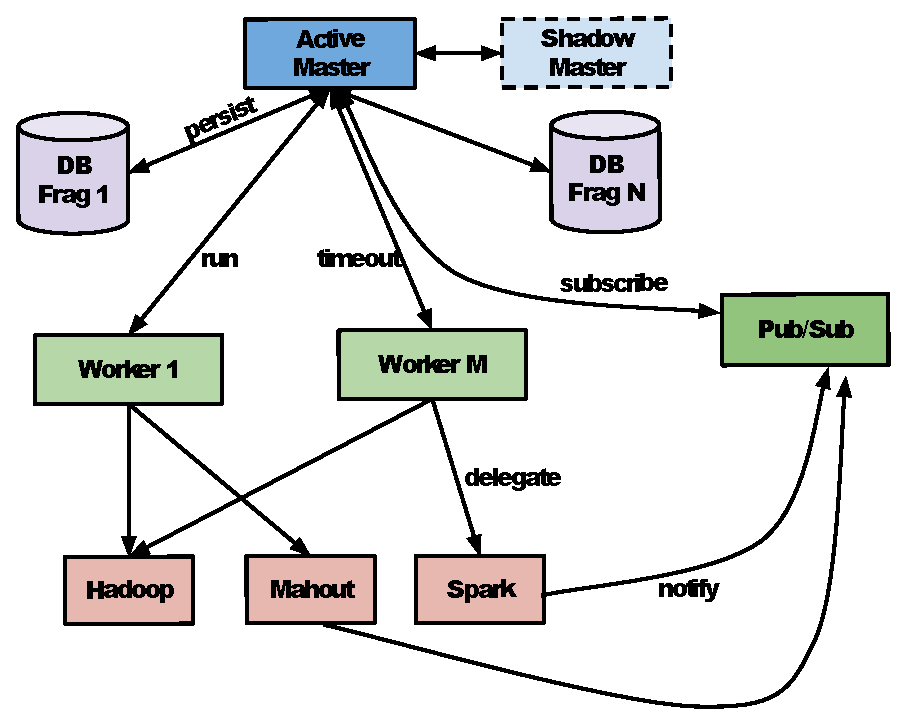
\includegraphics[scale=0.87]{DronDesign1}
\caption{Architecture Overview}
\label{fig:DronDesign1}
\end{figure}


For persisting the data we have chosen Erlang's builtin database, Mnesia. The main arguments for our decision are the fact that the database is well integrated with the programming language while others such as MySQL are not, it is easy to replicate on multiple machines and finally it provides two types of persistence (on disk as well as in main memory).


As one of our main goals is to build a fault tolerant system, we could not allow for any single point of failures. As a result, the master node has one or more hot-standby nodes. In case of a master node failure, one the other nodes is promoted to the a master role using a leader election algorithm.


While developing the system we have continuously evaluated its performance. This has allowed us to discover early on the bottlenecks, and more importantly, that the initial architecture was not be able to meet all the goals we have set for the system. In the following sections we will discuss in depth the various design changes and optimizations we have made in the iterative development process of Dron.

\section{Erlang Background}
Before we proceed with the explanation of the design, we have to briefly introduce several concepts about programming with Erlang/OTP. The code is divided into modules that may be either a plain or a behaviour module. The behaviours are formalizations of common patterns such as finite state machines, event handlers or servers. An example of such a behaviour is the \textit{Generic Server Behaviour} (\textit{gen\_server}) which implements the client-server relation. The model is characterized by a central server and an arbitrary number of clients that can send or request data from the server. As a result, the \textit{gen\_server} is a callback module that exports a pre-defined set of functions. Among them there are \textit{handle\_call} and \textit{handle\_cast}. The former must be implemented to handle synchronous requests from the clients while the later must be implemented for the requests that must be handled asynchronously. With the help of \textit{gen\_server} one may develop complex distributed systems modelled as a collection of servers and processes that communicate between them.


The second important Erlang/OTP concept we are introducing is the \textit{Supervisor Behaviour}. A supervisor is responsible for starting, monitoring and stopping a set of children processes. A common design pattern used in Erlang is to build supervision trees. With the help of the trees one may express the computation as a set of worker processes that are monitored by a set of supervisor processes. The pattern strongly encourages Erlang's philosophy which is to treat failures as the norm and not as the exception. By conducting the computation in state-less worker processes, the system can handle failures by simply allowing the supervisor processes to restart the computation in a different process.

\section{First Iteration}
Before we have started developing Dron we have considered various architectural solutions. The option we have chosen for our first iteration is presented in Figure \ref{fig:DronDesign1}. The system is centered around a multi-purpose master node that schedules jobs, manages workers, filters event from a publisher/subscriber system and persists data.


Since the master node was playing a central role, we had to make sure that its failure would not make the entire system unavailable. We have considered three solutions for this problem. Following we will briefly explain the advantages and disadvantages of each one of them.

\subsubsection{Single Master With a Database}
Each action conducted by the master (e.g. job instance creation, worker alive message) must be saved in a database that is replicated on several other machines. Upon master's failure the maintainer of the system must launch a new master node on one of the machines containing a replica of the database. The node would first reconstruct an in-memory state from the database after which it would proceed to schedule jobs.


The main advantage of this design is its simplicity. Having the master node on a single machine does not require the developer to think and handle consistency and network partition issues. On the other hand, it can not offer good availability in case of failures. One would have to manually start the master on a different machine and the process may take a long time as the entire state would have to be reconstructed from the persistent storage. Lastly, the master may quickly become a bottleneck as it is required to write all the operations to the database.

\subsubsection{Multiple Masters Organized in a ZooKeeper Quorum}
ZooKeeper~\cite{Zookeeper} is a service for coordinating processes, maintaining configuration information, providing distributed synchronization and group services. It allows distributed processes to coordinate with each other via a shared hierarchical namespace that is kept in-memory. Moreover, with the help of the namespace API one may implement more powerful primitives such as: configuration management, leader election, group membership, locks, double barrier, distributed queues etc.


The name space provided by ZooKeeper is similar to a standard file system. The main difference is that in ZooKeeper each node can have data associated with it as well as children. The API provides simple primitives to create, delete, read and write data atomically to the ZooKeeper nodes. On top of that the system also supports the notion of ephemeral nodes. These nodes are created by the client systems and exists until the client explicitly deletes them or until the session is terminated (e.g. client failure) when ZooKeeper automatically removes them. Lastly, the system also provides watches to allow clients to be notified of changes without requiring them to poll.


ZooKeeper can be used to perform two important tasks within our system: atomic broadcast and leader election. By creating a quorum of ZooKeeper nodes, we can delegate the master election protocol to ZooKeeper. The quorum will be responsible for detecting and handling node failures, network partitions and related events. When a service will be considered to be dead, its connection with ZooKeeper will be invalidated, its ephemeral nodes will be synchronously removed from the name space and the events will be distributed to watchers.


\begin{figure}[h]
\centering
\includegraphics[scale=0.65]{ZooKeeper}
\caption{ZooKeeper usage example}
\label{fig:ZooKeeper}
\end{figure}

With the help of ZooKeeper's atomic broadcast protocol (Zab~\cite{Zab}) and its name space Dron would be able to distribute its state over several machines. Figure \ref{fig:ZooKeeper} shows how it can be achieved. Every worker node can create and ephemeral node under the \textit{/workers} node. Thus, in case of a failure or a network partition, every watcher will be notified. Similarly, we can create a hierarchy for jobs, in which for each instance we will create a children under the node representing the job.


Despite the fact that ZooKeeper is a system that has been used in production for a long time we chose not to build Dron around it because of the following reasons:
\begin{itemize}
\item{}
There is no API support for Erlang. As a result, we would have had to implement a service that would receive requests from Dron and forward them to ZooKeeper. This would add much complexity to our system and at the same time it would decrease maintainability. 
\item{}
A three server ZooKeeper quorum scales up to around 20 000 requests per seconds. If we assume an average of 10 requests per job instance, then the system will only be able to handle around 2 000 job instances per second. This would not be enough to meet the goals we have outlined for Dron.
\end{itemize}

\subsubsection{Shadowed Master}
The third design we have considered is the one presented in Figure \ref{fig:DronDesign1}. Similarly to the first architecture, it consists of a master node that coordinates the scheduling, monitors workers and persists data. However, in this design the master node has one or more hot-standby nodes. When a node failure happens, a leader election algorithm picks and informs which hot-standby node will be responsible for coordinating from there on. Over the next few subsections we will study the implementation in more detail.

\subsection{Modules}
Figure \ref{fig:DronErlang} provides an overview of the main modules implemented in the first iteration and the way they interact. Following, we briefly describe the role of each module:

\begin{figure}[h]
\centering
\includegraphics[scale=0.65]{DronErlang}
\caption{Implementation Overview}
\label{fig:DronErlang}
\end{figure}

\begin{itemize}
\item{}
\textbf{dron} - the module implements the \textit{application} behaviour and
it is responsible for starting and stopping the whole framework. This involves starting the database nodes, starting the scheduler and finally attaching worker nodes.
\item{}
\textbf{dron\_mnesia} - the module is responsible for starting and stopping Mnesia on a set of given nodes. While starting the nodes, it makes sure to create and distribute the database tables over them and to setup the data replication.
\item{}
\textbf{dron\_sup} - the module implements the \textit{supervisor} behaviour. It
is responsible for monitoring and restarting the scheduler and the pubsub module in case of a failure. However, if these processes fail more than once every 60 seconds, then the supervisor will choose not to restart them and it will terminate the entire system. We have chosen not to allow for more often failures because we believe that the processes implementation should be reviewed if they are crashing regularly.
\item{}
\textbf{dron\_api} - is the entry point to Dron. It exports methods to register/unregister jobs and to kill job instances. We expect users, to only use this module while interacting with the system.
\item{}
\textbf{dron\_scheduler} - is the most important module from the system. It has many responsabilities such as: schedule jobs, create job instances, persist data to the database, maintain timeout timers, check for dependencies and handle job failures.
\item{}
\textbf{dron\_pool} - the module is managing all the Dron workers. It does so by implementing the \textit{gen\_server} behaviour and by allowing other modules to add or remove workers. It also uses Erlang's capabilities to monitor failures of distributed nodes. Lastly, the module also implements the policy that dictates job instance to worker assignments.
\item{}
\textbf{dron\_db} - is a module that exports all the operations involving the database that are required by other modules.
\item{}
\textbf{dron\_pubsub} - manages the entire communication with the publisher/subscriber system. It implements the \textit{gen\_server} behaviour with the help of which it manages connections to the publisher/subscriber. Moreover, it is also responsible for providing a clean and simple to use API for other modules (e.g. dron\_worker) to publish messages and start consumers. 
\item{}
\textbf{dron\_event\_consumer} - is the default job instance event subscriber. It consumes all the events published on a queue and it notifies the scheduler about the job instances state changes.
\item{}
\textbf{dron\_worker} - the module implements the \textit{gen\_server} behaviour and exports all the operations required to run and manage job instances. An instance of this module is executed on every worker machine. In this way the scheduler can delegate tasks to every worker machine.
\end{itemize}


In the following subsections we will give more implementation details about the most important modules.

\subsection{Scheduler}

\subsubsection{Description}
The scheduler represents the core of the system. Following, we will briefly explain the way we have implemented each important feature of the scheduler:


\begin{itemize}
\item{}
\textbf{Create and manage job instances} - the node maintains a timer for each job. When the timer is triggered, it creates a job instance whose description is saved in the database. The job instance will go through a series of states that are represented in Figure \ref{fig:JobStates}. First, it will be in \textit{waiting} state until its dependencies are satisfied. Following, the scheduler will look for a worker machine onto which to run the instance. After it sends the description of the instance to the selected worker node, the scheduler changes the state of the instance to \textit{running}. From there on, the job instance can transition to one of the following final states: \textit{failed}, \textit{succeeded}, \textit{timeout} and \textit{killed}.
\item{}
\textbf{Maintain timers} - the scheduler is also responsible for creating and managing three types of timers. The first type of timers is the one which is used to trigger when the next run of a job should occur. These timers are created when a newly job is registered.


The second type of timers are instantiated when new job instances are created. They are to be triggered when the dependencies of an instance have not been satisfied until a pre-specified timeout. We have taken great care to make sure that these timers are cancelled when a job instance starts running.


The last type of timers are the ones that are going to be triggered when a job exceeds its maximum allowed running time. When one of these timers is triggered it sends a message to scheduling process. Upon receipt of the message, the scheduler makes sure that the job instance is stopped and that its state is updated to \textit{timeout}.


In an initial version, we have stored all the timers in the state of the gen\_server implemented by the scheduler. However, as we learned more about Erlang we have found out that the state is completely copied whenever it is modified. Since the state changes at least whenever a state transition happens, we have tried to look into alternatives to this solution. We have come across \textit{ets} which is a built-in term storage. It provides the ability to store data in an Erlang runtime system, and to have constant time access to it. The data is organized into dynamic tables, with each one of them being created by a process. When the creator process terminates, the table is automatically destroyed. Thus, in our case the tables storing the timeouts are created by the process running the gen\_server and are shared with all the processes launched by the scheduler. This change gave the scheduler a significant speed improvement and allowed it to scale more.
\item{}
\textbf{Instantiate dependencies and check their state} - an important role of the scheduler node is to make sure that job instances are run only  when their dependencies are satisfied. It achieves by first collaborating with the \textit{dron\_language} module to transform every dependency specification from the form given by the user to information that exactly describes job instances (i.e. job name, running time).


The instanciated dependencies are written to the database as well as into an in-memory structure. We have chosen to store the data into the RAM as well because it is accessed on numerous occassions by the scheduler. In this way we have managed to reduce the load on the database and the scheduling delay.
\end{itemize}


\begin{figure}[h]
\centering
\includegraphics[scale=0.85]{JobStates}
\caption{Job instance state transitions}
\label{fig:JobStates}
\end{figure}


\subsubsection{Failures}
One of our main goals was to provide a system that is able to continue running under various failure scenarios. In this subsection we will study several failure situations that could have affected the scheduler node.


Developing the system with a single scheduler process was a relatively easy task to achieve. The timers corresponding to each job were all stored in the memory of the node. However, the failure of the machine on which the scheduler was running would have had catastrophic consequences (i.e. all the job timeout, dependency timeout timers would have been lost). Thus, we had to make sure that scheduling would continue even in case of master machine failure. As it can be seen in Figure \ref{fig:DronDesign1}, we have decided to have one or more hot-standby schedulers. Each one of them tries to have the same in-memory state as the active scheduler. Thus, whenever the master machine would fail, one of the secondary schedulers would take up its place. However, this introduced a whole new problem that our system had to tackle. The following subsection will describe the problem and briefly describe how we managed to solve it.


\subsubsection{Leader Election}
On a master scheduler failure, every secondary node is competing to become responsible for scheduling. The problem has been extensively studied in the literature as the \textit{leader election problem}. Many solutions have been devised for it that work only under a specific set of constraints (e.g. synchronous system, ring network). Thus, in the following paragraphs we will describe the requirements of our system.


Having designed the system such that it does not support network partitions (because Mnesia does not handle well such situations) implies that our leader election algorithm does not have to cater for such situations. Moreover, since the communication between nodes is conducted with the help of TCP/IP, we can say that it is reliable and that no messages are lost. However, the algorithm should be fault-tolerant with respect to failing and restarting processes and nodes. It must terminate and guarantee that a single node is elected as the leader and that every other node knows whether it was elected as a leader or not.


An algorithm that meets our requirements is the \textbf{Bully Algorithm} which has been presented in ~\cite{LeaderElection1, LeaderElection2}. The algorithm assumes that each process has an unique identifier and that there is a way to monitor processes failures. Thus, when a process P observes that the coordinator no longer replies to messages it holds an election as follows: 

\begin{enumerate}
\item{}
P sends an election message to all the processes with bigger identifiers.
\item{}
If P does not receive any response within a given time, then it wins the election and becomes the new leader.
\item{}
If one of the processes with a bigger identifier receives the message, then it replies to P and, finally, it takes over the election.
\end{enumerate}


The Bully algorithm also handles the case when a process known to be failed manages to come back up. Thus, when the process restarts, the algorithm will hold an election. If the new process has the highest identifier then it will win the election and be declared as the new leader.


An adjusted version of the algorithm was implemented in ~\cite{GenLeader}. The solution was implemented in Erlang and it extensively makes use of Erlang's abilities to detect failed processes. The major modification that was made to the algorithm, was to avoid conducting an election whenever a process with a smaller identifier that the leader is started. The implementation is available via the \textit{gen\_leader} behaviour. It can be seen as an extension of the standard \textit{gen\_server} behaviour. Listing \ref{lst:GLeader} briefly describes the additional functions the behaviour exports. With their help we have succeeded in supporting leader election and state replication among a set of scheduler nodes.



\newpage
\begin{lstlisting}[language=Erlang,caption={gen\_leader behaviour},
label={lst:GLeader}]
 %% Called in the leader process when it is elected. The synch node will be
 %% broadcasted to all the other nodes.
 %%
 %% @spec elected(State, Election, undefined) -> {ok, Synch, State}
 elected(State, Election, undefined)

 %% Called in the leader process when a new node joins the pool. The synch node
 %% will be sent to the node.
 %%
 %% @spec elected(State, Election, Node) -> {ok, State}
 elected(State, Election, Node)

 %% Called in all pool nodes except the leader. Synch is the message the leader
 %% has sent when it has been elected.
 %%
 %% @spec surrendered(State, Synch, Election) -> {ok, State}
 surrendered(State, Synch, Election)

 %% Handle synchronous calls made to the leader. Upon completion of handling the
 %% message, the leader can broadcast a term to all the other nodes.
 %%
 %% @spec handle_leader_call(Request, From, State, Election) ->
 %%    {reply, Reply, Broadcast, State} | {reply, Reply, State} |
 %%    {noreply, State} | {stop, Reason, Reply, State} | {stop, Reason, State}
 handle_leader_call(Request, From, State, Election)

 %% Handle asynchronous calls made to the leader. Upon completion of handling the
 %% message, the leader can broadcast a term to all the other nodes.
 %%
 %% @spec handle_leader_cast(Request, State, Election) ->
 %%    {ok, Broadcast, State} | {noreply, State} | {stop, Reason, State}
 handle_leader_cast(Request, State, Election)

 %% Handle the broadcast messages sent by the leader.
 %%
 %% @spec from_leader(Request, State, Election) ->
 %%    {ok, State} | {noreply, State} | {stop, Reason, State}
 from_leader(Synch, State, Election)

 %% Called in the leader when nodes go down.
 %%
 %% @spec handle_DOWN(Node, State, Election) ->
 %%    {ok, State} | {ok, Broadcast, State}
 handle_DOWN(Node, State, Election)
\end{lstlisting}

\subsubsection{Gen Leader}
We have used the \textit{gen\_leader} behaviour to implement the active-shadow master relationship. The adaptation from a scheduler using a \textit{gen\_server} to the new version consisted of three main steps. Firstly, we have changed all the handle\_call and handle\_cast functions to be implemented with a new version that broadcasts information to the shadow nodes. In most of the cases the information is almost identical to the data that is passed while calling the server.


Secondly, we have implemented the functions required to handle the broadcasts made by the active node. The purpose of these methods is to create the same in-memory state as in the active scheduler. By using the data we are sending in the broadcast messages (e.g. timer rate and timeout) we are creating timers with the same triggering time as in the active master.


Lastly, we had to make sure that all the Erlang messages that are sent directly to the scheduling process do not change its state. To achieve this, we have updated the dependencies checking mechanism to only use the API provided by the gen\_server behaviour.

\subsection{Pool}
The pool module is responsible for holding all the information related to the worker nodes. Thus, its API provides methods to add and remove workers. When a a worker is added, the pool first checks if it can communicate with the new node. Following, it updates its in-memory state and the database with information about the node.


Another important role of the pool is to monitor the status of the workers. Under a general model there is no way to implement node monitoring. In \cite{CAP}, Brewer has stated the following conjecture, that later was proven to be a theorem: it is impossible for a distributed system to simultaneously provide all three of the following guarantees:

\begin{itemize}
\item{}
\textbf{Consistency} - all the nodes have the same view of the data at the same time.
\item{}
\textbf{Availability} - guarantees that every request will receive a response in a timely manner.
\item{}
\textbf{Partition Tolerance} - the system continues to operate well when arbitrary messages are lost or even when two or more parts of it can not communicate at all.
\end{itemize}


As Dron was designed to be deployed within a single data center, we expect network partitions to rarely happen. Furthermore, because Mnesia was not designed to handle partitions we have chosen to do the same in our worker monitoring implementation. We have chosen to use Erlang's ability to monitor its own nodes. The feature communicates with the watched nodes at a given time interval, using a connection it maintains. If one of the workers fails or if a network partition occurs, the pool receives a \textit{nodedown} message that contains information about the failed node. Upon receipt of the message the pool updates its in-memory state and the persistent database.


The pool server is also in charge with deciding on which machine every job instance will be run. We have opted for simplicity and we have implemented our workers to be slot based. Thus, whenever a job instance is started, the number of free slots is decreased, and whenever the instance finishes, the number of free slots is increased. The algorithm picking the worker assignments implements a greedy strategy. Every time it simply picks the worker that has the biggest number of free slots. If two workers have the same amount of free slots then the algorithm picks the one that is stored first in the internal data structure.  We expect the solution to achieve good load balancing in practice due to the heterogeneity of the jobs. However, if later we will see that this is not the case we could extend the pool to monitor the resource utilization of the workers as well. Based on the additional information we can assign workers by taking in mind their load as well. The strategy could be implemented as a multi-dimensional knapsack, with each dimension representing a resource such as: memory, cpu, etc.


Since the pool module is an important component of Dron, we do not want to let our system fail when the pool would temporarily crash. As a result, we have chosen to implement a recovery procedure to be called in case of an unexpected failure. This procedure reconstructs the state of the server from the database. Considering we do not expect to have more than 500 Dron worker nodes, the process of reconstructing the state should be quick and it should not significantly increase the scheduling delay.

\subsection{Publisher/Subscriber}
The publisher/subscriber system is a crucial part of Dron as well. It is used by all the workers and external frameworks to publish events of interest to the scheduler. In our current implementation they are mostly job state change events. However, we believe that as the system will mature more events will be published. For example, the frameworks could publish information about their state (e.g. load, free map/reduce slots) such that the Dron will be able to optimize scheduling. Following, we describe the systems we have considered to use and the way we have finally integrated the publisher/subscriber in the scheduler.

\subsubsection{Kafka}
Kafka is a distributed publish-subscribe messaging system. It has been designed to provide high-throughput (i.e. hundreds of thousands of messages per second), persistent messaging, support for partitioning messages accross multiple Kafka servers and distributed messages consumption.


The messages are published to a topic by a producer when they are sent to a Kafka broker. On the other end, several processes can act as consumers. Each consumer process belongs to a consumer group and each message is delivered exactly to one process within a consumer group. Thus, with the help of groups one can distribute the load over a set of consumers by putting them into the same group, or one can send every message to every consumer by not allocating more than a process to each consumer group.


Kafka makes extensive usage of the local file system for persisting messages. The system writes all the data to a persistent log (on the file system), allowing the operating system to decide when to flush it. Moreover, it allows the users to specify a flush policy which controls how often the data is written to the persistent disk. The frequency of data flushes also limits the amount of messages that will be lost in case of a broker failure. For example, a policy of a flush per second in a broker that handles N messages per second guarantees that no more than N messages will be lost in case of a failure. The arguments provided by the developers against an usual in-memory storage and flush include the high memory overhead of Java objects and garbage collector inadequacy in handling big heaps.


Compared to other publisher/subscriber systems, Kafka does not provide rich filtering semantics. This is the result of the way in which messages are persisted. In order to improve throughput the engineers have decided not to use the standard solution for storing data (BTrees). The argument is that even tough BTrees operations are O(log N) in theory, they do not perform well in practice as they may require several disk seeks. A single disk seek can be performed at a time and it usually takes 10ms. Thus, they have used a persistent queue which is modelled as simple reads and appends to files.


While Apache Kafka meets most of our requirements we have decided not to use it in our system because of the following reasons:

\begin{itemize}
\item{}
The API is too restrictive and it does not allow message filtering. Thus, the only way to make sure that consumers are only receiving messages they are interested in is to define a queue for each consumer.
\item{}
It has been developed in Java and it only provides a Java API. As a result we would had to use an Erlang to Java communication tool called JInterface even tough we were unsure of its stability. 
\end{itemize}

\subsubsection{RabbitMQ}
RabbitMQ is an open source implementation of the Advanced Message Queueing Protocol (AMQP) developed for message-oriented middleware. The system introduces several concepts described bellow:

\begin{itemize}
\item{}
\textbf{Producer} - a program that sends/publishes messages.
\item{}
\textbf{Consumer} - a program that receives messages published on a queue.
\item{}
\textbf{Exchange} - receives messages from producers and it forwards them to queues. A message can be appended to a particular queue, a set of queues or even discarded. The routing of the messages is influenced by the type of the exchange (e.g. direct, topic, headers, fanout).
\item{}
\textbf{Queue} - acts as a temporary storage point for messages. It receives messages published by multiple producers and it allows many consumers to receive them.
\end{itemize}

The system runs a RabbitMQ broker which is a grouping of one or more nodes running the Erlang application. The broker is responsible for maintaining the queues, the exchanges, and for routing the messages to the consumers. The state of the broker is replicated accross all the Erlang nodes within the cluster. However, the messages sent to a queue are only stored on the machine that created the queue.


A broker consisting of a single node does meet our fault-tolerance requirements. The failure of the node implies lack of availability. Even worse, no matter if persistent queues are used, some messages may be lost because of buffering. Luckily, RabbitMQ has a feature that allows the system to be available even in the case of multiple nodes failure and decreases the chances of lost messages. The aforementioned properties can be obtained by using the active/active high availability feature for queues. It works by mirroring the queue on multiple nodes. One of the nodes is declared as the master of the queue while the others become slaves. All operations on a queue other than publishing are applied to the master first and subsequently are broadcasted by the master to the slaves.


New nodes may join the broker cluster at any time. When a node joins the cluster, some queues may decide to use it as a slave. When this happens the node starts receiving messages published to the queues for which it acts as a slave. However, it will not try to get any of the messages that have been previously published and not consumed. As a result the slave is unsynchronised up to the moment when all the old messages are drained.


Node failures are handled by a mirrored queue according to the type of the node:
\begin{itemize}
\item{}
\textbf{Slave Node} - the metadata is updated and the master remains the same. The messages are not lost and the operations continue as before except that the replication factor of the queue has decreased by one.
\item{}
\textbf{Master Node} - the eldest slave is promoted to be the new master because it has the highest chance of being synchronized with the master. If there is no slave that is fully synchronized with the master then the messages stored only on the master are lost.
\end{itemize}


Lastly, we would like to point that RabbitMQ does not tolerate network partitions well as a consequence of their usage of Mnesia. This shortcoming does not affect our system as Dron was built using Mnesia. Hence, it is vulnerable to network partition failures as well.


Having seen the features that RabbitMQ has we decided to use it as a publisher/subscriber in our system. Another reason for which we have picked it is that it was implemented in Erlang. Thus, we have managed to avoid any inter language communication and to reduce our development time. 

\subsubsection{Usage}

Dron is using RabbitMQ to send and receive all the events related to job instances states. Thus, when a job instance is run, the system decides if  a Dron worker or an external framework is responsible for sending the state change events. For example, a MapReduce job requires Hadoop to publish the events while for a simple shell script they are published by a Dron worker. As a result the system has a fanout exchange named \textit{dron\_events} that is available to receive messages. A valid message contains the job instance id and the new state encoded as an JSON object. The have chosen to use JSON in order to allow external frameworks to use the same exchange if they want. In Chapter \ref{chap:Integration} we will explain how to integrate a new framework with Dron, how to create new exchanges and make use of RabbitMQ's filtering features.


The module that is responsible for creating exchanges, starting consumers and publishing messages is \textit{dron\_pubsub}. It is implemented as an Erlang gen\_server. On its initialization it creates a connection to RabbitMQ and it setups all the exchanges and consumers that have been specified in the dron\_config module. Subsequently, it can be used by other modules (e.g. dron\_worker) to publish messages. Listing \ref{lst:DronPubSub} contains a part of the code written to created the default exchanges and consumers. On lines 3 and 4 we first create a connection to RabbitMQ and then we open a channel. Following, on lines 6-8 we setup all the exchanges declared in the \textit{dron_config} module. In the next step (lines 9-13) we bind the consumers to the queues they have been declared to be interested in. Finally, on line 15 we store in the state of the \textit{gen\_server} the connection and the channel we have previously created.\newpage


\begin{lstlisting}[language=Erlang,caption={Publisher/Subscriber usage},
label={lst:DronPubSub}]
% Function called on the initialization of the server.
init([]) ->
    {ok, Connection} = amqp_connection:start(#amqp_params_network{}),
    {ok, Channel} = amqp_connection:open_channel(Connection),
    % Setup all the exchanges declared in the config module.
    lists:map(fun({Exchange, Type}) ->
                      setup_exchange_intern(Channel, Exchange, Type) end,
              dron_config:exchanges()),
    % Setup all the consumers declared in the config module.
    lists:map(fun({Module, Exchange, RoutingKey}) ->
                      start_consumer_intern(Channel, Module, Exchange,
                                            RoutingKey)
              end, dron_config:consumers()),
    % The connection and the channel are part of the state of the server.
    {ok, #state{connection = Connection, channel = Channel}}.

start_consumer_intern(Channel, Module, Exchange, RoutingKey) ->
    #'queue.declare_ok'{queue = Queue} =
        amqp_channel:call(Channel, #'queue.declare'{}),
    Binding = #'queue.bind'{queue = Queue,
                            exchange = Exchange,
                            routing_key = RoutingKey},
    #'queue.bind_ok'{} = amqp_channel:call(Channel, Binding),
    proc_lib:start_link(Module, init, [self(), Channel, Queue]).

setup_exchange_intern(Channel, Name, Type) ->
    Exchange = #'exchange.declare'{exchange = Name, type = Type},
    case amqp_channel:call(Channel, Exchange) of
        #'exchange.declare_ok'{} -> ok;
        _                        -> error
    end.
\end{lstlisting}


\subsection{Worker}
The Dron worker servers have been designed to be as simple as possible. They are state-less servers that only act as a proxy between the master node and the machine. Every worker receives commands to run job instances upon which it spawns operating system processes in which the instances are executed. Depending on how it was instructed the server notifies the master of an instances state change by publishing an event message using the publisher/subscriber system.


We have chosen to design the workers as state-less in order to reduce the complexity of the implementation. Thus, whenever a worker failure occurs, the monitoring pool simply acknowledges it and it redistributes the instances to the remaining worker nodes. The tasks are re-executed without increasing their retry number as the failure was caused by an unexpected cause.

\subsection{Issues Encountered}
During the development of the system We have chosen to refine Dron's architecture by constantly testing the system for bottlenecks. In this subsection we describe the performance issues that have affected the first version of Dron and the optimizations we have implemented.


The benchmark we have used in our bottleneck driven development is testing the schedulers ability to handle as many job instances as possible every second. As we can see from Table \ref{tab:Dron1JI}, during the first few tests we have conducted, Dron was able to run up to around 100 job instances per second. At this point the system would crash with an error stating that too many database tables are open.


Since the database was causing the first bottleneck, we have decided to optimize the system's usage of it. We have gone through every single transaction that Dron was performing and we have studied the possibilities of removing or changing them such that they use more fine grained locking. By using dirty reads we have managed to reduce the number of transactions executed per job from nine to seven. As a result the system could now scale up to approximatively 120 job instances per second. However, at bigger loads it would crash with the same error message as in previous case.


Upon further investigation about Mnesia's internals, we have found out that during a transaction the database creates a temporary in-memory table called ets. The Erlang runtime environment places a default limit of 1400 on the number of tables that can exist simultaneously. This basicaly limited the number of transactions that can be carried at the same time. However, after we increased the limit to 65536 tables, Dron was able to schedule around 300 job instances until it would crash without any error message.


Following we have discovered that the new crashes were caused by the code we have added into the scheduler to monitor the delay. The code was processor intensive. The moment we have improved it Dron was able to scale up to around 400 job instances per second.


\begin{table}[h]
\centering
\begin{tabular}{|l|p{7.5cm}|}
\hline
\textbf{Jobs/second} & \textbf{Issue}\\ \hline
100 & Too many database tables open. \\ \hline
120 & Too many database tables open.\\ \hline
300 & The scheduler crashes with no reason.\\ \hline
400 & Writing and reading from the workers table takes too long.\\ \hline
500 & The machine can not handle the load.\\ \hline
\end{tabular}
\caption{Scalability issues encountered by the first architecture as optimization were conducted}
\label{tab:Dron1JI}
\end{table}


In order to detect what was causing the newly found bottleneck we extensively profiled the code. While doing so, we have discovered that reading and writing information to the database about the workers state (e.g. number of free/used slots), was significantly increasing the scheduling delay. To solve the issue, we have decided to maintain in-memory information about workers. While this may increase the state of the scheduler it also has an important advantage: it reduces the load on the database by allowing the scheduler to only go to the database during write operations. 


After the last optimization the system was able to handle around 500 job instances per second. At this point, the big load would cause the Mnesia transactions to race for access and to continuously retry until they would reach the maximum number of retries. Moreover, the 6Gb of RAM that our testing machine had and the Dual-Core 2.5GHZ CPU would be used up to almost 100\%.


The tests and the optimizations we have conducted inspired us to embark on the daunting task of improving Dron's architecture. In the following section we will study the improvements we have made to the system. 

\section{Second Iteration}
In the previous section we have presented the bottlenecks we have encountered during the development of the first version of Dron. Based on our experiments we have decided to change the architecture of the system in order to be able to meet our goals. In the next few subsections we will discuss the changes we have made.

\subsection{Description}
Despite all the optimizations we have made to the scheduler's implementation and to our usage of the database, we did not managed to scale the system to handle more than 500 job instances per second. Furthermore, we believe that most of the optimizations that could still be conducted will not bring major performance improvements. The fact that the resources of the machine running the scheduler are completely utilized under such a load supports our belief. As a result we have decided to change the architecture of the system such that multiple scheduler nodes can be run in parallel.


In Figure~\ref{fig:DronDesign2} we can see an overview of the new Dron architecture. When comparing it to the previous design, one can observe that a new type of node has been introduced. The coordinator is the new central module of the system. Its main role is to distribute the load among the running schedulers. The other components have suffered changes that are not obvious from the figure. In the following few paragraphs we will briefly explain the changes every important module has gone trough.

\subsubsection{Coordinator}
The coordinator is a new module of the system that acts as a thin monitoring and managing layer. It is the only component that has complete information about the running worker and scheduler nodes. Moreover, whenever someone wants to add a new node to Dron, it calls the appropriate coordinator function and from there on, the node launches and monitors the new component.


Similarly, to the previous version of the scheduler, we have chosen to increase the fault-tolerance of the node by adding several hot-standby nodes. This has been achieved by implementing the \textit{gen\_leader} behaviour. The in-memory state of the coordinator consists mostly of information about the worker scheduler assignments and information about the schedulers. Thus, the active coordinator only has to broadcast information to the shadow nodes when the state of one of the scheduler or worker nodes changes.


As we will see in Subsection \ref{subsec:WorkersBalancing} the coordinator also requires the scheduler nodes to send information about their state, at a specific time interval. By simply using the default methods Erlang provides for monitoring, we could not send data defined by us. Thus, we were forced to implement our own heartbeat based monitoring system. The implementation will be explained in the following section.


Lastly, the coordinator is also responsible for load balancing the jobs accross the active schedulers. We have chosen to use the Erlang's default hash function to achieve it. However, if upon further investigation we will observe that the function does not perform well under various loads, we can change it with our own implementation. We could implement the consistent hashing~\cite{ConsistentHashing} algorithm. The function has been proven to perform well even when the number of hashing buckets changes. In our case this would be when schedulers are added or removed or when they fail.

\subsubsection{Scheduler}
We have managed to reuse most of the code while adapting the scheduler to the new architecture. However, during the process we have also found out that the supervisors processes we have used, had to be completely changed. This was due to the fact that the supervisors have been developed to be used within the same node. While they may behave well in monitoring process on the same machine they do not give any availability guarantees while being used in a distributed setting. This issue was overcome using our own heartbeat protocol which will be presented in the next subsection.


Another important change was made in the way the system handles dependency checking. Up to now, the single scheduler had information about all the dependencies. Moreover, it would receive state change events for every single job instance. In the new implementation the coordinator only forwards the state change events to the node that is responsible for the scheduling of the job. As a result, the schedulers may not be aware when some of the dependencies are satisfied. We have solved this issue by adding to the scheduler the possibility of receiving messages about satisfied dependencies. Lastly, we have also changed the coordinator such that when it receives a state change event it forwards the message to all the possible interested schedulers.


\begin{figure}[h]
\centering
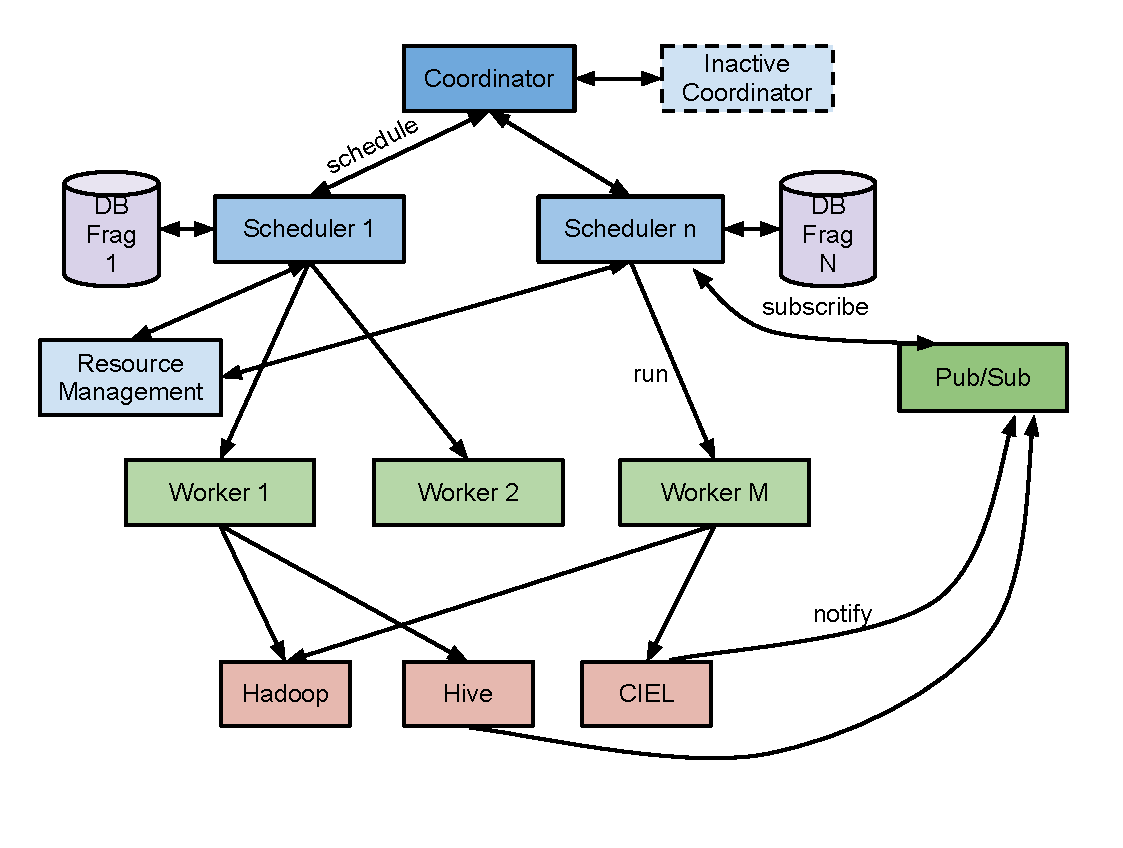
\includegraphics[scale=0.75]{DronDesign2}
\caption{Architecture Overview}
\label{fig:DronDesign2}
\end{figure}

Once we have distributed scheduling on several machines by running many schedulers at the same time we have created an entire new set of challenges to be tackled. Each one of the following subsections will describe a challenge and the solution we are providing for it.

\subsection{Workers Balancing}
\label{subsec:WorkersBalancing}
Having several schedulers running in parallel introduces the problem of deciding who will be responsible of worker monitoring and assignment. Following, we discuss the three options we have considered:

\begin{enumerate}
\item{}
The coordinator is responsible of managing all the workers.
\item{}
Each scheduler is monitoring all the workers and can run a job instance on any
of them.
\item{}
Fragment the pool of workers such that each scheduler has control over a subset
of workers.
\end{enumerate}


The first solution can easily be achieved by adapting the worker pool from our first implementation. However, we believe it has several shortcomings. First, the coordinator will quickly become a bottleneck as it will have to answer to all the worker requests made by schedulers. Lastly, the scheduling delay will increase because for each job instance we would have to do a call to the coordinator. The call will be synchronous and will get the name of the worker on which the job instance should be run.


The second option reduces the load on the coordinator. However, it still has a bottleneck, which is the database. For each worker we persist the number of occupied slots/resources. Thus, we have to update them whenever a job instance is run. This will force us to fragment the workers table over several machines in order to be able to handle the load. As a result, a big percentage of worker related writes that every scheduler makes, will be conducted on fragments situated on remote nodes. The solution also makes it difficult to provide Service Level Agreement (SLA) for high priority jobs as they will be run on any machine with any other potentially unfair (i.e. cpu and memory intensive) jobs.


The third option solves the bottlenecks discussed above by allowing each scheduler to manage its own worker pool. However, this solution has a big disadvantage as a scheduler may become a hot spot and run out of worker resources. We have managed to solve this shortcoming by developing self balancing worker pools.


The algorithm is composed of the following steps:
\begin{enumerate}
\item{}
At a given interval of time every scheduler computes a value representing the load of its workers.
\item{}
Based on the computed load and its policy every scheduler decides if it requires more workers or if it can offer several.
\item{}
Every scheduler sends its request/offering to the coordinator node. The content of a message is presented in Table \ref{tab:WorkersBalancing}.
\item{}
The coordinator reassigns offered workers to the schedulers that need more.
\end{enumerate}


\begin{table}[h]
\centering
\begin{tabular}{|l|p{6.0cm}|}
\hline
\textbf{Message} & \textbf{Description}\\ \hline
\{SchedulerName, \{request, Number\}\} & A scheduler is requesting Number workers
\\ \hline
\{SchedulerName, \{offer, Number\}\} & A scheduler is offering Number workers
\\ \hline
\end{tabular}
\caption{Worker Pools Balancing Protocol}
\label{tab:WorkersBalancing}
\end{table}


\begin{figure}[h]
\centering
\includegraphics[scale=0.8]{DronWorkers}
\caption{Workers Balancing}
\label{fig:DronWorkers}
\end{figure}


Figure \ref{fig:DronWorkers} presents a simple example of workers balancing. At the beginning the pool running at node dron1 has two workers and the pool running at node dron2 has one worker. Subsequently, every scheduler is computing the load on its pool. The load indicates that the pool from node dron1 is wasting resources while the one from node dron2 is requiring more. Thus, the first pool offers a worker, while the other one requests a worker. Lastly, the coordinator decides that Worker 2 will be reassigned to the pool running on node dron2.


We have developed the self balancing workers feature to be flexible. Thus, it can be configured the time interval at which every scheduler should compute and send its offerings/requests to the coordinator. Moreover, we allow every scheduler to have its own sharing policy. Currently, we are supporting three types of policies:

\begin{enumerate}
\item{}
\textbf{Low Priority} - the scheduler offers workers when its load is not very high and requires when it is utilizing almost all of its resources. In our simple slot-based schedulers we have chosen to offer workers when less than 30\% of the slots are used and to request for extra workers when more than 90\% are used.
\item{}
\textbf{Medium Priority} - the scheduler is less willingly to offer workers and will request for more sooner that the Low Priority scheduler. It requests for extra workers when the load reaches 80\% and it offers workers when the load is less than 20\%.
\item{}
\textbf{High Priority} - the scheduler almost never offers any workers (only when load is smaller than 10\%). Moreover, it requests workers as soon as the pool reaches a load of 70\% or more.
\end{enumerate}


We believe that scheduler policies are an important feature of Dron as they give guarantees in handling important jobs. For example, an important team within a company (e.g. ads analytics) could just deploy their own scheduler that manages a set of high specification, purposely configured machines. Their scheduler could be high priority or use a no share policy which will make sure that almost none of their workers will be offered to other schedulers.


We would like to point that experiments could be conducted to study how the scheduler priorities behave under different job traces. These tests could also be used to fine-tune the thresholds for each priority. However, we leave the experiments as future work as they are not central to the project.

\section{Summary}
When we have designed Dron, the main goal was to build a scalable job scheduler system. We have started with a simple design centered around a single node scheduler. After some preliminary evaluation of the system, we have gained a better understanding of the bottlenecks which affected it. Despite the optimizations conducted and explained in the current chapter we have not managed to make the single node architecture to scale up to our goals.


We acknowledge the fact that there may be optimizations to be implemented in our single node architecture. Nevertheless, we believe that they can not bring the scalability improvement needed to meet our requirements. We have briefly explained the architectural changes we have made in order to solve this shortcoming. The evaluation must further show if our decisions have strengthen the performance of the system enough to meet the goals we initially set.


\chapter{Integrating Frameworks}
\label{chap:Integration}
\section{Introduction}
An important goal of the system was to provide simple ways of integrating different types of frameworks with the scheduler. In this section, we discuss the possibilities of achieving the aforementioned and the difficulties we have encountered while adapting several systems.


When Dron is starting a job in an external system, it must have a way of monitoring the job's state. In other words, it has to be informed when the job completes successfully or when it fails. The scheduler is providing to the developers, two solutions to detect the mapping between a Dron job instance id and an external job. In both cases the framework running the job must send notification events (e.g. job completion, job failure). The events can be sent using an implementation of AMQP (RabbitMQ). The content of the events will depend on which one of the following two solution the developer is choosing:


\begin{enumerate}
\item{}
Change the framework to support job parameters. Thus, every time when Dron runs a job instance, it will pass the dron job instance id as a parameter to the framework. This approach will allow the external system to send events on a common AMQP queue (e.g. dron\_events). Following, the messages received on the queue are forwarded to a subscriber (Dron Events Filter) which will parse them and notify the Dron Coordinator.


The solution is suitable for frameworks that already support job parameters or for the ones that do not require extensive redesign to have this functionality. The advantage of the solution is that the mapping between dron job instance and the job running in the framework is explicitly handled. Thus, the developer does not have to make any changes in Dron's code base.

\item{}
Adapt the system to notify on events (e.g. job completion, file creation) and provide a module that filters the events. In this case, the scheduler does not have to explicitly send the dron job instance id to the external framework. Thus, the solution is suitable for the cases when passing parameters to a job is not available or difficult to achieve. However, the developer must be careful to encode enough information in the messages so that the event filter module will be able to infer the mappings between dron job instances and externally executed jobs.


The approach is also suitable for handling dependencies on external resources (e.g. MySQL tables). Whenever a MySQL table will be created by a Dron job or an external user, an event will be published on a queue (e.g. dron\_mysql\_events). The module provided by the developer will be automatically subscribed to the queue and it will receive the events. Its role is to inform the coordinator about which resources have been satisfied. Finally, the coordinator will run the jobs that depend on the recently satisfied resource.
\end{enumerate}

\begin{figure}[h]
\centering
\includegraphics[scale=0.75]{AdaptFramework}
\caption{Possibilities of Adapting Frameworks}
\label{fig:AdaptFramework}
\end{figure}


Figure \ref{fig:AdaptFramework} depicts the two ways of integration external systems with Dron. The Spark framework has been adapted to support job arguments. Thus, when \textit{Worker 1} is running \textit{job instance 1} (i.e. a Spark job) it will also pass the job instance id to the framework. Subsequently, when the job finishes, Spark publishes an event consisting of a JSON object. As showed in Table \ref{tab:DronEvents} the object contains the Dron job instance id and its state. Lastly, the event is received by the default Dron event filter which will inform the coordinator.


\begin{table}[h]
\centering
\begin{tabular}{|l|p{5.9cm}|}
\hline
\textbf{Events} & \textbf{Description} \\ \hline
\{``job\_instance:''1'',''state'':''succeeded''\} &
Sent when the job started by Dron job instance 1 has successfully
completed\\ \hline

\{``job\_instance:''1'',''state'':''failed''\} &
Sent when the job started by Dron job instance 1 has failed \\ \hline

\{``job\_instance:''1'',''state'':''killed''\} &
Sent when the job started by Dron job instance 1 has been killed \\ \hline
\end{tabular}
\caption{Dron Events}
\label{tab:DronEvents}
\end{table}


\textit{Job instance 2} is a job that creates a file in the Hadoop Distributed File System (HDFS). Since the file system has been integrated using the second method, \textit{Worker N} does not have to pass the job instance id to it. However, an event filter has been provided to handle HDFS events published on \textit{dron\_hdfs\_events} queue. They are JSON objects composed of the name of file/directory and the event that affected it (e.g. created, deleted).


The following sections will detail the changes we made to every framework and the challenges we were faced with.

\section{Hadoop MapReduce}
MapReduce has become the core framework for performing data or process intensive tasks. We decided to adapt Hadoop version 0.20.2 using the first method. The system provides a listener interface for users to implement and register with the scheduler. In Listing \ref{lst:MRAdapt} we present an extract of the listener we have implemented. The \textit{jobUpdated} method is called with an event whenever the state of any job changes. From that event we are extracting the status of the job. On lines 12,18,24 we are checkig if the job is in one of the three states: succeeded, failed or killed. In the case of each state we are publishing a JSon message on the Dron publisher/subscriber queue.


The piece of code described above will sit at the core of the Hadoop scheduler. We had to make sure that it does not significantly increase the load on the scheduler. Moreover, we also wanted to make sure that dron events are published even in case of transient failures (e.g. network spike, queue temporarily down) as the loss of an event could lead up to job instances timeout. The aforementioned goals have been achieved with the help of a thread pool and a connection pool.

\newpage
\begin{lstlisting}[language=Java,caption={Job State Listener},
label={lst:MRAdapt}]
public class JobStateChangeMonitor extends JobInProgressListener {
  private final Dron dron;
  private final String exchangeName;

  public JobStateChangeMonitor(Dron dron, String exchangeName) {
    this.dron = dron;
    this.exchangeName = exchangeName;
  }

  public void jobUpdated(JobChangeEvent event) {
    JobInProgress jobInProgress = event.getJobInProgress();
    if (jobInProgress.getStatus().getRunState() == JobStatus.SUCCEEDED) {
      JSONObject jsonObject = new JSONObject();
      jsonObject.put("job_instance",
          jobInProgress.getJobConf().get("dronJobInstanceId", "-1"));
      jsonObject.put("state", "succeeded");
      publish(jsonObject.toJSONString());
    } else if (jobInProgress.getStatus().getRunState() == JobStatus.FAILED) {
      JSONObject jsonObject = new JSONObject();
      jsonObject.put("job_instance",
          jobInProgress.getJobConf().get("dronJobInstanceId", "-1"));
          jsonObject.put("state", "failed");
          publish(jsonObject.toJSONString());			
    } else if (jobInProgress.getStatus().getRunState() == JobStatus.KILLED) {
      JSONObject jsonObject = new JSONObject();
      jsonObject.put("job_instance",
          jobInProgress.getJobConf().get("dronJobInstanceId", "-1"));
      jsonObject.put("state", "failed");
      publish(jsonObject.toJSONString());
    }
  }

  private void publish(String message) {
    dron.publish(exchangeName, message);
  }
}
\end{lstlisting}


Figure \ref{fig:HadoopAdapt} provides an overview of our solution. The \textit{Dron} class is responsible for creating the pools for and publishing messages. Knowing that creating a new Connection for every job event is a slow process we decided to implement a \textit{Connection Pool}. It is responsible for managing a set of connections. Thus, whenever the scheduler wants to publish a message it can acquire a connection from the pool. Subsequently, when the message has been sent, it has to release the connection.


Sending a message to a remote machine is a slow operation that should not keep the \textit{JobStateMonitor} listener busy. A simple solution would spawn a new thread whenever a message must be published. However, this approach does not work at the scale at which Hadoop is receiving job state change events because creating a new thread is an expensive operation. As a result, we decided to use a fixed size thread pool. Whenever a message must be published, Dron can simply reuse one of the available threads. 


We handled transient network failures by using exponential backoff while sending each message. Listing \ref{lst:MRAdapt2} presents our simple implementation. First, we try to send the message. If we do not succeed in publishing it, the thread will sleep for a predefined amount of time (e.g. 100 milliseconds). Subsequently, the we try to send the message again. If we do not succeed on this attempt as well then we double the amount of time for which we sleep. As a result the thread attempts to publish a message until a maximum sleep time is reached.

\begin{figure}[h]
\centering
\includegraphics[scale=0.7]{HadoopAdapt}
\caption{Hadoop Integration Design}
\label{fig:HadoopAdapt}
\end{figure}

Finally, we would like to point that the adaption was not as difficult as we were expecting. The only challenges were to find the exact places where changes were required, and to understand how the code works at a fine grained level. Both of them were the result of working with a system compromising of more than 300 000 lines of code not adhering to a standard coding style.


\section{Spark}
Being aware of Hadoop's weaknesses exhibited while running iterative jobs, we have decided to integrate the Spark~\cite{Spark} cluster computing system as well. The Scala based framework provides primitives for in-memory cluster computing. Thus, iterative jobs can quickly access the data instead of writing and reading it from the distributed file system as in Hadoop.


\newpage
\begin{lstlisting}[language=Java,caption={Event Publisher}, label={lst:MRAdapt2}]
for (long sleep = 100; sleep <= MAX_SLEEP_MS; sleep <<= 1) {
  try {
    Channel channel = channelPool.acquireChannel();
    channel.basicPublish(exchangeName, "", null, message.getBytes());
    return;
  } catch (InterruptedException e) {
    LOG.error("Thread could not sleep");
  } catch (IOException e) {
    LOG.error(e);
    try {
      Thread.sleep(sleep);
      Connection connection = connectionPool.acquireConnection();
      channelPool.addNewChannel(connection);
      connectionPool.releaseConnection(connection);
    } catch (InterruptedException e1) {
      LOG.error("Thread could not sleep");
    } catch (IOException e2) {
      LOG.error("Could not add new channel", e2);
    }
  }
}
\end{lstlisting}


Being confronted with a relatively small project we have decided to adapt it such that it can receive Dron job instance id whenever a new Spark job is run. This has been achieved by enhancing two classes modelling Spark jobs. Subsequently, we had to provide a RabbitMQ publisher for Spark. Even tough there is no RabbitMQ client library for Scala we managed to easily reuse the Java implementation. Lastly, we had to adjust the Spark scheduler to send job failure/success events to Dron.\\


\begin{lstlisting}[language=Java, caption={Additions to the Mesos scheduler:
whenever a job completes, a JSON object is constructed and published according to
the job's state.},label={lst:Spark}]
if (job.hasFailed() == true) {
  val jsonMap: Map[String, Any] =
          Map("job_instance" -> dronInstanceId,
               "state" -> "failed")
  val jsonObject = new JSONObject(jsonMap.toMap)
  dron.publishMessage(jsonObject.toString())       
} else {
  val jsonMap: Map[String, Any] =
          Map("job_instance" -> dronInstanceId,
              "state" -> "succeeded")
  val jsonObject = new JSONObject(jsonMap.toMap)
  dron.publishMessage(jsonObject.toString())       
}
\end{lstlisting}


We believe that Spark will not be used as extensively as the MapReduce framework. Thus, we chose to implement a simple solution in which we use the scheduler thread to publish messages. However, if a performance drop is observed one could simply implement a solution based on channel and thread pools. Listing \ref{lst:Spark} provides an extract of the changes we had to make in the scheduler. Similarly, to the Hadoop's case we check for the state of the job on line 1. If the job has failed then we construct a JSON object on lines 2-5 which is later published (line 6). We treat the other case equivalently.

\section{Mahout}
We believe that being able to run machine learning computations on top of Hadoop has allowed users to solve a set of problems at a scale bigger than ever. For example, in Chapter \ref{chap:Recommendation} we will show how to easily build a scalable recommendation engine using Dron, Mahout and Hadoop.


The machine learning library is implemented as a driver program. Thus, we were able to easily find the entry point to the system and to detect the places where changes were required. The driver receives the address of the RabbitMQ host, the name of the AMQP exchange and the Dron job instance id corresponding to the Mahout job as command line arguments. Since the driver runs on the machine where it has been started (i.e. on dron workers) and only manages a single job, we did not have to implement a more complex solution that uses thread pools. Thus, we only had to monitor the state of the job and to publish an event when it would change.


Listing \ref{lst:Mahout} represents an extract of the code we have added. The if statement makes sure that an event is published only for a job that has received the RabbitMQ host, exchange and the Dron job instance id. 
\\

\begin{lstlisting}[language=Java,caption={Excerpt of Mahout Adaptation},
label={lst:Mahout}]
if (host != null && exchange != null && dronJobInstanceId != null) {
  Dron dron = new Dron(host);
  dron.publish(exchange, dron.buildJsonString(dronJobInstanceId, status));
  dron.close();
}
\end{lstlisting}

\section{Summary}
In the previous sections we have demonstrated the possibilities of integrating external frameworks with Dron. We believe that the two options do not require complex changes in the other systems. Even so, in some cases we may want to quickly run several jobs in a new framework without going through the hassle of adapting it. This is possible as long as we make sure that the Unix command that triggered the task exits only when the computation is finished. In this way Dron will be able to know about the computation's exit signal. The disadvantages of this approach is that Dron will not have much information about the state of the job and that worker resources will be wasted by occupying slots with waiting processes. Despite these we have chosen to run Hive queries using this approach as it saved us the time we would have spent changing Hive. 


Finally, we would like to point that we believe that the integration should be taken a step further. The frameworks would sent information about their state such that Dron can adapt the execution order of the jobs.



\chapter{Evaluation}
\label{chap:Evaluation}
In this chapter, we will start by evaluating the scalabilaty of our scheduler. We first compare it to anoter workflow scheduler (Oozie). Following, we evaluate the behaviour and performance of Dron under high loads.


In order to test different scheduling strategies, we construct a benchmark which is modelled after real-world computations. Lastly, we discuss the results and we study how the utilization of the cluster changes under four scheduling strategies.

%\section{Workers Balancing}
%\subsection{Protocol Frequency}
%TODO: Graph on how I've decided on the frequency.
%TODO: Compute the load it poses on the coordinator.
%\subsection{Low Priority Policy}
%TODO: Graph showing how I've decided on the values. Show under various loads.
%\subsection{Medium Priority Policy}
%TODO: Graph showing how I've decided on the values. Show under various loads.
%\subsection{High Priority Policy}
%TODO: Graph showing how I've decided on the values. Show under various loads.


\section{Dron's Scalability}
The two main questions we set ourselves when evaluating the performance of the system are:
\begin{itemize}
\item{}
How is the job scheduling delay affected as the number of jobs is increasing?
\item{}
How many jobs can the system handle at a time before its performance significantly degrades?
\end{itemize}


We answer them by first comparing Dron to the most similar system that has been built and that currently represents the state of the art. Following, we analyse Dron's behaviour under heavy load and we discover its bottlenecks.

\subsection{Dron and Oozie}
Oozie~\cite{Oozie} is a job scheduler developed by Yahoo for the Hadoop framework. In certain aspects it is similar to Dron, as it allows users to create workflows composed of multiple MapReduce or Pig jobs.


In order to answer the first question mentioned above we studied how the scheduling delay is affected by the increase of the number of scheduled jobs. First, we scheduled 100 no operation jobs to be run at the same time. In Figure \ref{fig:OozieDelay} and \ref{fig:DronDelay} we have constructed the histograms of the scheduling delay incurred by each system. From the figures we can observe that \textbf{Oozie can handle on average 3.57 jobs per second and that the average scheduling delay is 15.33 seconds}. Since the average MapReduce completion time is of 395 seconds~\cite{ClusterFailure} we believe that Oozie's delay is quite significant as it ads another 3.88\% extra running time to every job. On the other hand, \textbf{Dron has managed to schedule the jobs in under 1 second and with an average delay of 0.78 seconds}.


\begin{figure}[h]
\centering
\includegraphics[scale=0.50]{ooziedelay}
\caption{Histogram showing Oozie's scheduling delay on a test with 100 jobs}
\label{fig:OozieDelay}
\end{figure}


\begin{figure}[h]
\centering
\includegraphics[scale=0.50]{drondelay}
\caption{Histogram showing Dron's scheduling delay on a test with 100 jobs}
\label{fig:DronDelay}
\end{figure}


Following, we have tested how the scheduling delay is affected if we increase the number of jobs in our benchmark to 1000. In figure \ref{fig:OozieDelayBig} we present the histogram representing the number of jobs scheduled every 20 seconds. From it we can observe that Oozie is scheduling around 195 jobs every 20 seconds for the first 100 seconds. However, after that we can see a big drop in performance. The scheduler can not keep up with the load and as a result it only manages to run approximatively 50 jobs every 5 minutes. As a result, the last 17 jobs of the 1000 are scheduled after 1028 seconds from the beginning of the benchmark.


We have also run the same test using Dron. In Figure \ref{fig:DronDelayBig} we have built the histogram representing the number of jobs that are scheduled every second. As we can see from it, the system has successfully scheduled the jobs in under 0.9 seconds and with an average delay of 0.35 seconds.


\begin{figure}[h]
\centering
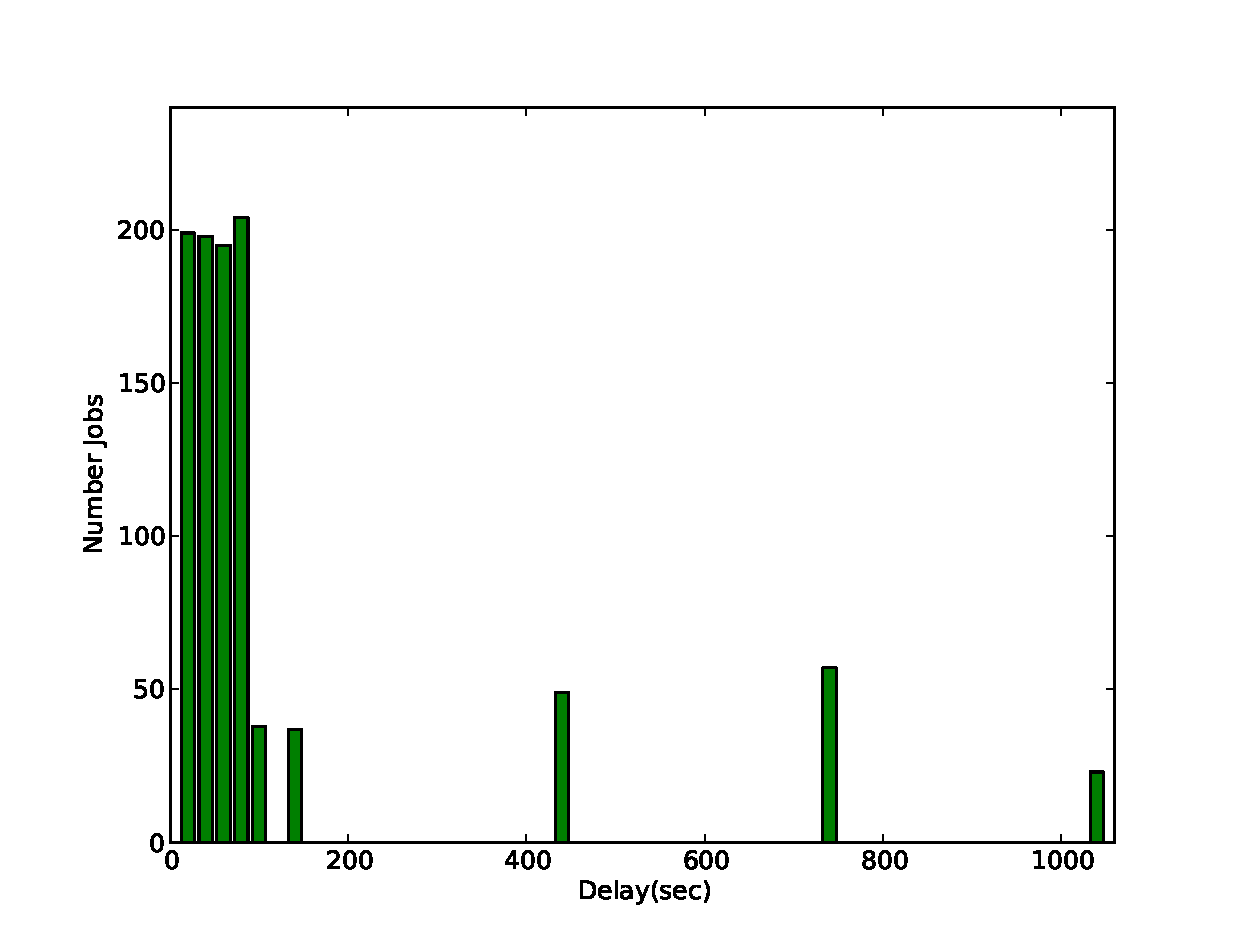
\includegraphics[scale=0.50]{ooziedelaybig}
\caption{Histogram showing Oozie's scheduling delay on a test with 1000 jobs}
\label{fig:OozieDelayBig}
\end{figure}


\begin{figure}[h]
\centering
\includegraphics[scale=0.50]{drondelaybig}
\caption{Histogram showing Dron's scheduling delay on a test with 1000 jobs}
\label{fig:DronDelayBig}
\end{figure}


Having conducted the above described tests we have shown that Dron's scheduling overhead is much smaller than Oozie's. Moreover, Dron scales better when the number of jobs is increased. On top of that, the maximum number of non-empty jobs Oozie can run at the same time is bound by the number of Map slots available in the Hadoop cluster. The fact that the biggest Hadoop deployments have around 30 000 Map slots, makes Oozie unable to handle more than approximatively 10 000 jobs at the same time. From the author's own experience this is not enough to handle the needs of a company such as Facebook, that relies on large data analysis.


Oozie's limitation comes for the fact that every job specification is first copied onto HDFS and subsequently is run as a Map task even tough it is a simple Java program. While we understand that the developers of the system have concentrated on simplicity, we believe that Oozie is not able to meet many companies scalability requirements. Moreover, it does not provide good fault-tolerance as it was designed to be run on a single machine, without any secondary machine to act as a hot standby.


\subsection{Scheduling Delay}
In order to better understand the performance of Dron, we have built a benchmark that stresses the system's ability to handle events happening at the same time (e.g. jobs completing or jobs being scheduled). The test is composed of identical jobs that are simple \textit{sleep 0} Unix commands. This has allowed us to increase the number of slots on each worker to 20 000, and as a result, to decrease the number of worker machines required for the test. Moreover, the simple jobs do not change the benchmark's focus, which is to study the scalability of the Coordinator, Scheduler and Database nodes.


The test starts by registering 500 periodic jobs. They are expected to run every 10 seconds. Subsequently, at every 30 seconds, the benchmark registers another 500 jobs. The process continues, until the scheduling delay significantly increases or until the system crashes.


We have executed the benchmark on two deployment configurations. In the first setup, we have launched two EC2 large instances. One was used as a worker node and the other one was used to run the Dron Coordinator, Scheduler and Database. Before running the test, we have deployed our own monitoring software in order to have a better understanding of our machines status.


The system behaved well and had a scheduling delay of only one second up to a load of 250 jobs per second. After that, the delay increased to two seconds and, as the number of jobs grew, to 370 per second. However, at around 380 jobs per second the delay started to increase exponentially until the scheduler crashed. This was caused by the database's inability to scale up more, fact confirmed by the crash message: ``system\_limit, Cannot create an ets table for the local transaction store''.


In Figure \ref{fig:LatencyOneCpu} and \ref{fig:LatencyOneMem} we have plotted the CPU and memory usage of the machine on which we ran the Coordinator, Scheduler and the Database. The values, have been collected every 5 seconds from the beginning of the test until the end. From the graph on the left side we can see how the CPU utilization increased as we registered more jobs. The spikes are the result of the fact that we have not succeeded to uniformly distribute the jobs across the 10 seconds interval. The figure on the right shows that the memory usage was very low and that it did not increase by much as we registered more jobs. However, despite the relatively low resource utilization the scheduler has not been able to scale more.


Subsequently, we decided to test if the scalability of the system improves if we add more database and scheduler nodes. We have deployed Dron on 6 Amazon EC2 large instances. Four of them were used to run four schedulers and database shards, while the remaining two were used as worker nodes. Both in this setup and in the previous one we have setup a database replication factor of two. Under this configuration the system has successfully managed to scale up to 850 jobs per second. For each one of them the scheduling delay was under two seconds. However, the moment we increased the load beyond 850 jobs per second the delay started to exponentially increase. As in the previous cases, we have monitored the all the machines. The graphs plotting the load on the most busy scheduler machine can be found in Appendix \ref{chap:EvalQueries}.


\begin{figure}[ht]
\begin{minipage}[b]{0.5\linewidth}
\centering
\includegraphics[scale=0.35]{latency-one-cpu}
\caption{CPU usage on the machine running the Dron Coordinator, Scheduler and Database during the benchmark testing scheduling delay}
\label{fig:LatencyOneCpu}
\end{minipage}
\hspace{0.1cm}
\begin{minipage}[b]{0.48\linewidth}
\centering
\includegraphics[scale=0.35]{latency-one-mem}
\caption{Memory usage on the machine running the Dron Coordinator, Scheduler and Database during the benchmark testing scheduling delay}
\label{fig:LatencyOneMem}
\end{minipage}
\end{figure}


Lastly, we would like to point that Dron has been able to schedule 100 times more jobs per second than Oozie. Even so, we think that there are several tweaks that can be made to improve Dron's performance. For example, we could change Mnesia's hashing function to make it identical with the hashing function used by Dron to load balance jobs to schedulers. LinearHashing~\cite{LinearHashing} or ConsistentHashing~\cite{ConsistentHashing} would be two suitable algorithms as they are two hashing techniques suitable for environments in which the number of buckets changes often. In this way, we would be able to add extra schedulers and database nodes as the load increases. Moreover, every scheduler will only run jobs that are locally stored on its database shard. This will significantly reduce the load on the database and the latency of read operations.

\subsection{High Load}
Since Dron was built to schedule large data jobs we have also built a benchmark in order to evaluate how well it manages to handle many long running jobs. In this test we are interested to observe the system's ability to keep information about jobs that are running at the same time (e.g. timeout timers, monitoring processes). As a result we have tried to keep the jobs as simple as possible. Every job is a simple \textit{sleep 600} Unix command. This has allowed us to increase the slots on the worker nodes up to 10 000 and to ultimately use less machines.


The benchmark was executed using six EC2 large instances. One of the instances was used to run the Dron Coordinator, Scheduler and Database node. On each of the remaining machines we have deployed three Dron Worker nodes. Thus, the entire capacity of our deployment would sum up to 150 000 job slots.


The test first registers 25 000 periodic jobs. Every job is expected to run every 10 minutes. Subsequently, every 150 seconds, the benchmark registers an additional 25 000 periodic jobs. We have allowed the benchmark to register 150 000 which corresponds to the maximum amount of available job slots of our deployment. During the execution of the test we have sampled every 5 seconds the CPU and memory usage on the machine on which we ran the Dron Coordinator, Scheduler and Database nodes. The values we have collected are plotted in Figure \ref{fig:DronLargeCpu} and Figure \ref{fig:DronLargeMem}.


The left figure shows that the CPU usage was low through almost the entire duration of the test. The spike at the end was caused by the fact that the last two batches of 25 000 jobs have been scheduled to start exactly at the same time of the second run of the first two job batches. Even so, the CPU usage has barely reached 30\%. The figure on the right side plots the memory usage. From it we can see that the utilization steadily increases as the test proceeds. This is caused by two reasons:

\begin{itemize}
\item{More jobs are executed at the same time increasing the size of the state the scheduler is keeping in memory.}
\item{The size of the in-memory database increases as more job instances are created and executed.}
\end{itemize}

\begin{figure}[ht]
\begin{minipage}[b]{0.5\linewidth}
\centering
\includegraphics[scale=0.35]{dron-large-cpu}
\caption{CPU usage on the machine running the Dron Coordinator, Scheduler and Database during the high load benchmark}
\label{fig:DronLargeCpu}
\end{minipage}
\hspace{0.1cm}
\begin{minipage}[b]{0.48\linewidth}
\centering
\includegraphics[scale=0.35]{dron-large-mem}
\caption{Memory usage on the machine running the Dron Coordinator, Scheduler and Database during the high load benchmark}
\label{fig:DronLargeMem}
\end{minipage}
\end{figure}

The test we have conducted shows that the system is able to handle loads that the other currently publicly available large data schedulers can not. We believe that Dron's current scalability is enough even to meet the demands of the biggest companies relying on large data analysis.


\section{Scheduling Evaluation}
\label{sec:schedulingEvaluation}
In this section we demonstrate that by capturing the direct acyclic graph of job dependencies, Dron can use different scheduling strategies to improve the running time of the benchmark. There are two main questions we set ourselves when evaluating the different scheduling options:
\begin{enumerate}
\item{}
How is the overall running time of the benchmark affected?
\item{}
How does the resources utilization change with each strategy?
\end{enumerate}

In order to answer the above mentioned questions we construct a benchmark modelled after a real world scenario and we run it on a cluster. Before we proceed we would like to point that the scheduling strategies have not been developed with any fairness constraints in mind. We assume that the jobs in the benchmark do not have requirements in terms of job starting time. This problem could be solved by providing to the users the option of tagging jobs as prioritary (i.e. it must start at the given time) or not.

\subsection{Node Configuration}
We deployed Hadoop and Hive on a 21-node cluster. Each node is an Amazon EC2 large instance with 4 Compute Units, 7.5 GB of RAM and 850 GB of instance storage running Ubuntu 11.10 (Oneiric Ocelot). According to Amazon a Compute Unit has the equivalent CPU capacity of a 1.0-1.2 GHz 2007 Xeon processor. Using \textit{hdparm} we discovered that the hard disks deliver approximately 2400 MB/s for cached reads, 490 MB/s for buffered disk reads and 70 MB/s writing speed. With the help of \textit{iperf} we have also tested the network bandwidth and we have found it to be on average around 870 Mbits/s.


For our experiments we use Hadoop 0.20.2 and Hive 0.7.1 running on Java 1.6.0. We deployed the system with the default configurations settings: NameNode/JobTracker JVM heap size of 900 MB and DFS block size of 64 MB. One node was used as a NameNode/JobTracker and the remainder of 20 as TaskTrackers/DataNodes. Each nodes has been setup to execute at most 5 Map tasks and 2 Reduce tasks concurrently. Thus, our cluster has a total of 100 Map slots and 40 Reduce slots.

\subsection{Benchmark Description}
Our benchmark consists of 14 jobs. It has been built based on previous tests conducted by Pavlo et al. and Facebook engineers~\cite{PavloBenchmark, HiveBenchmark}. For each job we only give an overview of what its achieving. However, the interested reader can consult Appendix \ref{chap:EvalQueries} for listings of the Hive queries and the publicly available repository for the source code of the MapReduce jobs used.


As depicted in Figure \ref{fig:TestDAG} the benchmark is composed of 4 main categories of tasks. The first type of job is the ``Grep task'' which is described by the authors of the MapReduce framework to be ``representative for a large subset of real programs written by the users of MapReduce''\cite{MapReduce}. We have created two identical jobs to conduct this task. One is a MapReduce job and the other one is a Hive query. Both jobs are scanning through a 50GB data set generated using Pavlo's et al. benchmark. The data is composed of 100-byte records containing a 10 bytes unique key and a 90 bytes random value. The jobs are looking for a three-character pattern that is only found once in every 10 000 records.


\begin{figure}[h]
\centering
\includegraphics[scale=0.66]{TestDAG}
\caption{Direct acyclic graph of jobs used for benchmark}
\label{fig:TestDAG}
\end{figure}


The generated data is first loaded into HDFS text files using a Dron job. This phase is not included into the benchmark since it is a long step that does not stress any of Hadoop's resources (i.e. the duration of the loading phase depends on the reading speed of the disk where the data is initially stored). Following,
using the \textit{CreateGrepSel} Dron job we create a table into which the output of the Grep query will be inserted. Once this step is completed, we launch the
\textit{GrepH} query and the \textit{GrepM} MapReduce Job. The former is composed of 194 Map Tasks and the latter of 746 Map Tasks.


For the remaining tasks we have used Pavlo's et al. benchmark to generate a collection of HTML documents. Using the documents we have also generated two data sets that model log files of HTTP traffic. The first set stores for each page URL its page rank and the average duration visit. The second data set has been built to model user visits to a set of URLs. It contains information about the user(e.g. source ip, country code) and about its every website visit (e.g. date, ad revenue). For more information consult Table \ref{tab:TestHiveTables} which contains the schema of data sets we have used in our benchmark.


Similarly to Grep's data set, we did not include the data generating and uploading to HDFS into the benchmark. However, we have included 4 jobs that are responsible with creating the tables needed to store the output of the queries. \textit{CreateRankSel} is responsible for creating the table for a simple selection task. The purpose of the of the task is to filter the page URLs from the Rankings table that have a page rank bigger than a given value. As for all other categories of tasks we have created a job (\textit{SelRankH}) to run the Hive query and a job (\textit{SelRankM}) to run the MapReduce job. The number of Map and Reduce tasks required by each job can be seen in Table \ref{tab:TestHiveTables}.


The third category of tasks depend on the \textit{CreateUVJoin} job. They are tasks that perform complex calculations on the Rankings and UserVisists data sets.
In the first step the tasks lookup for the source ip that generated the most revenue within a given data range. Following, the tasks calculate the average page rank of the pages visited during the above mentioned interval. The difficulty of this category of tasks comes from the fact that the two different data sets (Rankings and UserVisits) must be scanned and joined together in order to compute the output. Thus, the tasks extensively stress the cluster's network and processing capabilities.


Finally, the fourth category of tasks depend on the \textit{CreateUVAgg} and \textit{CreateUVAd} jobs. \textit{AggUV} job calculates the total ad revenue generated for each source ip contained in the UserVisits data set, grouped by the source ip column. Upon's \textit{AggUVH} job completion, \textit{AdUVH} is started. The job computes the ad revenue generated everyday, grouped by the visit date. The aggregation tasks were designed to test the performance of parallel analytics on a single read-only table. The second aggregation task has been added in order to increase the depth of the direct acyclic graph. Thus, the workload better depicts loads that have seen by the author in his previous work experiences.
 

\begin{table}[h]
\centering
\begin{tabular}{|p{9.8cm}|p{2.9cm}|}
\hline
\textbf{Schema} & \textbf{Size} \\ \hline
\textbf{grep}(key varchar(10), field varchar(90)) & 500 million rows, 50GB \\ \hline
\textbf{rankings}(pageRank int, pageUrl varchar(100), avgDuration int) & 18.7 million rows, 1.1GB \\ \hline
\textbf{uservisits}(sourceIp varchar(16), destUrl varchar(100), 
visitDate date, adRevenue float, userAgent varchar(64), 
countryCode \mbox{varchar(3)}, languageCode varchar(6), 
searchWord varchar(32), duration int) & 160 million rows, 20.2GB \\ \hline
\end{tabular}
\caption{Benchmark Hive table's information}
\label{tab:TestHiveTables}
\end{table}

\subsection{Scheduling Strategies}
In this subsection we study four scheduling strategies that we have used in Dron in order to execute the benchmark described above. For each strategy we have ran the benchmark two times to make sure that the results are consistent.


In order to be able to conduct the tests we have extended Dron's job syntax. We give users the possibility to declare the number of Map and Reduce tasks required by each job. If the users provide this information, Dron can try to optimize the usage of the Hadoop cluster. Since the job scheduler is external to Hadoop it can only improve the utilization of the deployment by rearranging the order of the jobs. This solution can only bring advantages in cases when the cluster is overloaded. However, most of the companies that analyse big data are in this situation, fact confirmed even by our contacts at Facebook.


We overload our own cluster by starting at the same time, all the jobs described in the previous section. Thus, we successfully replicate real world scenarios in which jobs are queued up because of large computations.


Following we describe every strategy we have tested. For each one of them we also include a table detailing the order in which the jobs have been run. We have omitted the jobs that do not run Hadoop computations as they all are of short duration.


\subsubsection{1st Strategy}
In this setting the scheduler simply registers all the jobs at the same time. The jobs which depend on other jobs (e.g. \textit{AdUVHive}) will only be triggered when their dependencies succesfully complete. Table \ref{tab:DronTest1Jobs} contains information about the running order of jobs and their duration. From the table we can observe that MapReduce jobs are scheduled before all the Hive jobs. This is due to the computation that is conducted by Hive to transform the queries into MapReduce jobs and to their dependency on the jobs that create the tables.

\begin{table}[h]
\centering
\begin{tabular}{|l|l|c|c|}
\hline
\textbf{\#} & \textbf{Job Name} & \textbf{Start Time(sec)} & \textbf{End Time(sec)} \\ \hline
1 & Join UserVisits MapReduce & 37 & 863 \\ \hline
2 & Select Rankings MapReduce & 38 & 365 \\ \hline
3 & Aggregate UserVisits MapReduce & 47 & 365 \\ \hline
4 & Grep MapReduce & 197 & 473 \\ \hline
5 & Select Rankings Hive & 358 & 546 \\ \hline 
6 & Aggregate UserVisits Hive & 361 & 727  \\ \hline
7 & Join UserVisits Hive & 376 & 904 \\ \hline
8 & Grep Hive & 506 & 878 \\ \hline
9 & Aggregate Ads UserVisits Hive & 647 & 886 \\ \hline
\end{tabular}
\caption{Hadoop jobs running information for scheduling using 1st strategy}
\label{tab:DronTest1Jobs}
\end{table}


\subsubsection{2nd Strategy}
Using second strategy the scheduler prioritizes the jobs which have the highest direct acyclic graphs depending on them. The strategy was developed based on the hypothesis that the jobs situated on bigger level do not fully utilize the resources of the cluster. Our benchmark, excluding the jobs that create tables, has only one job with dependant jobs (\textit{Aggregate UserVisits Hive}). We expect it to be the first job to be run. However, in Table \ref{tab:DronTest2Jobs} we see that \textit{Grep MapReduce} is the first job executed. This is due to fact that \textit{Aggregate UserVisits Hive} depends on \textit{Create UserVisits Aggregate}. The dependency takes some time to be satisfied and on top of that even the starting delay of a Hive job is quite significant in our benchmark (i.e. it takes around 45 seconds to transform a Hive query into a series of MapReduce jobs). As a result the strategy runs a MapReduce job until the highest priority job is ready to be run. We expect this delay to be less important in large industry scale computations. However, we still consider it is an aspect to be kept in mind while refining strategies.


\begin{table}[h]
\centering
\begin{tabular}{|l|l|c|c|}
\hline
\textbf{\#} & \textbf{Job Name} & \textbf{Start Time(sec)} & \textbf{End Time(sec)} \\ \hline
1 & Grep MapReduce & 21 & 155 \\ \hline
2 & Aggregate UserVisits Hive & 168 & 454  \\ \hline
3 & Join UserVisits MapReduce & 169 & 810 \\ \hline
4 & Aggregate UserVisits MapReduce & 360 & 547 \\ \hline
5 & Grep Hive & 505 & 635 \\ \hline
6 & Join UserVisits Hive & 608 & 897 \\ \hline
7 & Select Rankings MapReduce & 674 & 848 \\ \hline
8 & Select Rankings Hive & 693 & 769 \\ \hline 
9 & Aggregate Ads UserVisits Hive & 685 & 777 \\ \hline
\end{tabular}
\caption{Hadoop jobs running information for scheduling using 2nd strategy}
\label{tab:DronTest2Jobs}
\end{table}


\subsubsection{3rd Strategy}
The third strategy is a refinement of the previous one. While running the benchmark we have observed that several jobs have multiple steps. For example the Hive query representing \textit{Join UserVisits Hive} is transformed into four MapReduce jobs. Figure \ref{fig:MultiJoin} details the requirements of the components of the multi-step jobs from our benchmark. This observation has encouraged us to allow users to specify information (i.e. number of Map/Reduce tasks expected) for every step of their Dron jobs. As a result the adjusted scheduler treats \textit{Join UserVisits MapReduce}, \textit{Aggregate UserVisits Hive} and  \textit{JoinUserVisits Hive} as priority jobs. Fact confirmed by the running order (Table \ref{tab:DronTest3Jobs}) we obtained while executing the benchmark.


We believe that with more time at hand we would be able to extend the scheduler with the ability to receive information about complex jobs from Hive and Hadoop. Subsequently, Dron could automatically use this to prioritize the jobs that have implicit dependant jobs.


\begin{figure}[h]
\centering
\includegraphics[scale=0.50]{MultiJoin}
\caption{Example of Dron jobs composed of multiple MapReduce jobs}
\label{fig:MultiJoin}
\end{figure}


\begin{table}[h]
\centering
\begin{tabular}{|l|l|c|c|}
\hline
\textbf{\#} & \textbf{Job Name} & \textbf{Start Time(sec)} & \textbf{End Time(sec)} \\ \hline
1 & Join UserVisits MapReduce & 29 & 836 \\ \hline
2 & Aggregate UserVisits Hive & 152 & 460  \\ \hline
3 & Join UserVisits Hive & 169 & 876 \\ \hline
4 & Aggregate UserVisits MapReduce & 252 & 504 \\ \hline
5 & Select Rankings MapReduce & 285 & 618 \\ \hline
6 & Select Rankings Hive & 469 & 537 \\ \hline 
7 & Grep MapReduce & 451 & 620 \\ \hline
8 & Grep Hive & 682 & 830 \\ \hline
9 & Aggregate Ads UserVisits Hive & 750 & 838 \\ \hline
\end{tabular}
\caption{Hadoop jobs running information for scheduling using 3rd strategy}
\label{tab:DronTest3Jobs}
\end{table}

\subsubsection{4th Strategy}
Lastly, we have tried to improve the previous strategy by delaying the run of a job that was determined to be prioritary. This strategy was developed from the hypothesis that the jobs situated at the higher levels of the benchmark's direct acyclic graph do not fully utilize the resources of the cluster. Thus, in order to balance computation, the scheduler has decided to postpone the \textit{Join UserVisits Hive} job.


\begin{table}[h]
\centering
\begin{tabular}{|l|l|c|c|}
\hline
\textbf{\#} & \textbf{Job Name} & \textbf{Start Time(sec)} & \textbf{End Time(sec)} \\ \hline
1 & Join UserVisits MapReduce & 26 & 852 \\ \hline
2 & Aggregate UserVisits Hive & 151 & 466  \\ \hline
3 & Grep MapReduce & 169 & 405 \\ \hline
4 & Select Rankings MapReduce & 398 & 657 \\ \hline
5 & Aggregate UserVisits MapReduce & 400 & 593 \\ \hline
6 & Grep Hive & 545 & 842 \\ \hline
7 & Select Rankings Hive & 658 & 697 \\ \hline 
8 & Join UserVisits Hive & 664 & 938 \\ \hline
9 & Aggregate Ads UserVisits Hive & 771 & 860 \\ \hline
\end{tabular}
\caption{Hadoop jobs running information for scheduling using 4th strategy}
\label{tab:DronTest4Jobs}
\end{table}


\subsection{Results}
In this section we study the results we have obtained while using the strategies outlined above. We have executed the benchmark twice for every scheduling order. This allowed us to verify that the running times were not affected by temporary network traffic spikes, virtual machines collocation (i.e. other resource intensive virtual machines situated on the same node) or many other possible transient failures.


In order to be able to answer the three questions mentioned in Section \ref{sec:schedulingEvaluation}, we have deployed our own resource monitoring system. This is because Amazon's CloudWatch only offers paid resource information at a minute interval. Our benchmark does not run for more than 17 minutes. The only few data points provided by CloudWatch would have not accurately captured the changes in the cluster utilization. As a result, we chose to manually deploy \textit{collectl} and to sample CPU, network traffic, disk and memory usage at a 5 second interval.

\begin{figure}[h]
\centering
\includegraphics[scale=0.40]{benchmark-duration}
\caption{Duration of benchmark depending on the strategy used while scheduling}
\label{fig:BenchmarkDuration}
\end{figure}


Figure \ref{fig:BenchmarkDuration} presents the duration of the benchmark while using the different scheduling strategies. We can observe that the 3rd strategy has a duration 3.1\% smaller than the first strategy and 6.6\% smaller than the 4th strategy. Moreover, while testing other scheduling orders that have not been covered in the report we have seen improvements of up to 10\%.


These results suggest that it is possible to reduce the duration of the benchmark by making use of the jobs dependency graph. For the test we have conducted it can be achieved by prioritizing the jobs that have the highest direct acyclic graphs depending on them and the jobs that are made of multiple steps. We would also like to point that this observation requires much more testing and refinement. The problem of scheduling is complex and it may be case that the 3rd strategy just schedules well the benchmark we have used.


\begin{figure}[ht]
\begin{minipage}[b]{0.47\linewidth}
\centering
\includegraphics[scale=0.36]{dron-cpu}
\caption{CPU usage on Dron node}
\label{fig:DronCpu}
\end{minipage}
\hspace{0.2cm}
\begin{minipage}[b]{0.5\linewidth}
\centering
\includegraphics[scale=0.36]{dron-mem}
\caption{Memory usage on Dron node}
\label{fig:DronMem}
\end{minipage}
\end{figure}

Following we try to answer the second question (how does the resources utilization change with each strategy?) by studying the data we have gathered about the nodes state. Figure \ref{fig:DronCpu} and \ref{fig:DronMem} plot the CPU and memory usage on the node that was used as a Dron coordinator, scheduler and worker. Due to the small size of the benchmark and to lack of computing power we have chosen to run all the above mentioned Dron components on the same machine. Even so, as the graphs point, the CPU and memory utilization were small. 


The plot representing CPU usage contains several spikes. Upon further analysis, we have discovered that they coincide with the starting times of the jobs that are running Hive queries. This is due to the fact that Hive queries are transformed to MapReduce jobs locally on the Dron machine. Except these spikes, the load on the machine is very low with the CPU usage rarely exceeding 5\%.


The memory footprint of the Dron components is very small. As it can be observer from Figure \ref{fig:DronMem} most of the memory is used by the operating system and by the benchmark jobs that are running on the node. As more jobs complete we can see the memory utilization decreasing down to 8\% for all the strategies.


\begin{figure}[ht]
\begin{minipage}[b]{0.47\linewidth}
\centering
\includegraphics[scale=0.36]{jtnn-cpu}
\caption{CPU usage on JobTracker/NameNode node}
\label{fig:jtnnCpu}
\end{minipage}
\hspace{0.2cm}
\begin{minipage}[b]{0.5\linewidth}
\centering
\includegraphics[scale=0.36]{jtnn-mem}
\caption{Memory usage on JobTracker/NameNode node}
\label{fig:jtnnMem}
\end{minipage}
\end{figure}

Figure \ref{fig:jtnnCpu} and \ref{fig:jtnnMem} are plotting the CPU and memory usage gathered from the EC2 node we have used to run the Hadoop \textit{JobTracker} and \textit{NameNode}. Since for large data standards our cluster is small, we have not seen any intensive resource utilization on this machine. As the plots show, CPU utilization almost never exceeds 10\% and memory utilization is constant at approximatively 9\%.


\begin{figure}[ht]
\begin{minipage}[b]{0.47\linewidth}
\centering
\includegraphics[scale=0.36]{avg-cpu-w}
\caption{Average CPU usage on worker nodes}
\label{fig:AvgCpuW}
\end{minipage}
\hspace{0.2cm}
\begin{minipage}[b]{0.5\linewidth}
\centering
\includegraphics[scale=0.36]{sd-cpu-w}
\caption{CPU usage standard deviation on worker nodes}
\label{fig:SdCpuW}
\end{minipage}
\end{figure}


Following, we have measured the resource utilization on the worker nodes. Figure \ref{fig:AvgCpuW} plots the average CPU usage accross all workers for every strategy. As we expected we can see that the worst strategy (4th) it is not using the CPU as much as the other strategies. After 570 seconds from the beginning of the benchmark the CPU usage drops to around 40\% and continues to be around that value for approximatively 60 seconds. On the other hand, For all the remaining strategies we do not see any big differences. Their overall CPU usage which is around 57\% for all of them. In order to get a better understanding we have also plotted the standard deviation of CPU usage across the workers. From this graph we can observe that for the first 500 seconds the computation is well distributed on all the workers nodes. Following, the standard deviation starts to increase as the final jobs do not make use of all the resources of the cluster. As we were expecting the average standard deviation for CPU utilization is bigger by 1.23 than the value observed for the 3rd strategy.


\begin{figure}[ht]
\begin{minipage}[b]{0.47\linewidth}
\centering
\includegraphics[scale=0.36]{avg-mem-w}
\caption{Average memory usage on worker nodes}
\label{fig:AvgMemW}
\end{minipage}
\hspace{0.2cm}
\begin{minipage}[b]{0.5\linewidth}
\centering
\includegraphics[scale=0.36]{sd-mem-w}
\caption{Memory usage standard deviation on worker nodes}
\label{fig:SdMemW}
\end{minipage}
\end{figure}


Figure \ref{fig:AvgMemW} and \ref{fig:SdMemW} plot the data we have gathered about the memory utilization on the worker nodes. Despite the variation in the running length of the benchmark we have not observed any big variations in the memory usage of the cluster. While scheduling the jobs using 3rd strategy we have seen an increase of 0.3\% in memory than while scheduling them with 4th strategy. However, we believe that this increase is to small to draw any conclusions upon.


\begin{figure}[ht]
\begin{minipage}[b]{0.47\linewidth}
\centering
\includegraphics[scale=0.36]{avg-net-w}
\caption{Average network usage on worker nodes}
\label{fig:AvgNetW}
\end{minipage}
\hspace{0.2cm}
\begin{minipage}[b]{0.5\linewidth}
\centering
\includegraphics[scale=0.36]{avg-dsk-w}
\caption{Average disk usage on worker nodes}
\label{fig:AvgDskW}
\end{minipage}
\end{figure}

Lastly, we have also measured the disk and network utilization. While computing the average network read and write speed (Table \ref{tab:NetSpeed}) we have observed a correlation with the duration of the benchmark. In order to better understand the similarity we have studied how many of the Map tasks are conducted using local data, tasks failure rates and percentage of tasks ran preemptively by the framework (Appendix \ref{chap:EvalQueries}). The findings did not hint to any reason for the difference in network usage. The disk utilization plotted in Figure \ref{fig:AvgDskW} has also shown better usage during the run with the 3rd strategy. In this case the disks have read/written on average an extra 2 MB/s than during the run using 1st or 2nd strategy.

\begin{table}[h]
\centering
\begin{tabular}{|l|c|c|c|c|}
\hline
\textbf{Strategy} & \textbf{1st} & \textbf{2nd} & \textbf{3rd} & \textbf{4th} \\ \hline
\textbf{Network Usage (MB/s)} & 9.91 & 9.52 & 9.2 & 10.74 \\ \hline
\end{tabular}
\caption{Average Network Utilization on Worker Nodes}
\label{tab:NetSpeed}
\end{table}


%\section{Dron's Fault Tolerance}
%\subsection{Goals}
%\subsection{Worker Failures}
%\subsection{Scheduler Failures}
%\subsection{Coordinator Failures}
%\subsection{Other Failures}


\section{Discussion}
Our experiements have shown that Dron scales better than other current existing workflow schedulers. With a bit of extra development time to remove existing bugs and to do few optimizations the system will be able to meet the needs of most companies relying on large data analysis. Following, we have also tested and evaluated four scheduling strategies. We have observed that one is performing better than the others. However, we think that many more tests should be conducted in order to study how the strategy performs under different scenarios.


We are aware that there are things to be improved in Dron's design. However, we believe that even as it is, the system is offering much flexibility. For example, by being able to run several schedulers at the same time the engineers can experiment with various strategies and more importantly change them without any downtime. Another good design decision we have made is that we provide two ways of integrating external frameworks with Dron. In this way, the engineers can choose the solution which is the most easy for them to implement. Nevertheless, we also think that several architectural decisions may create problems. For example, even if the coordinator node is just a thin layer, we expect it to become a bottleneck under heavy job loads.


Some of Dron's features can not be easily evaluated. For example, it was important for the system to provide a rich enough dependencies language. Since there is no way to quantify simplicity or language's expressiveness, we have decided to simply show that interesting system can be achieved with it. In Chapter \ref{chap:Recommendation} we show how to build a scalable recommendation engine using Dron, Hadoop and Mahout.


Finally, we would like to point that testing the system has proven to be much more difficult than anticipated. Firstly, we were faced with many problems while generating the data for the benchmark (e.g. hardcoded operating system dependencies in open source code, difficult to adapt implementation). Secondly, it took us few weeks just to correctly deploy Hadoop, Hive and Oozie on Amazon EC2. Despite all the automation bash and Python scripts we have written, the deployment process still consists of approximatively 25 steps.


\chapter{Recommendation Engine Based on Dron and Mahout}
\label{chap:Recommendation}

\section{Description}
In this chapter, we show how it is possible to build a scalable recommendation system with the help of Dron, Mahout and Hadoop. Developing such a system normally requires an effort equivalent to few person-months. However, by using multiple frameworks, we show that it is possible to be achieved in only several hours. Our solution is based on the description given in~\cite{RecommenderSystem}.

The recommendation system meets the demands of websites that have the following characteristics:

\begin{itemize}
\item{the items are not changing often (e.g. every few hours)}
\item{the number of users is significantly bigger than the number of items}
\item{the recommendations do not have to update in real-time}
\end{itemize}


An example of a website that has these properties would be a music discovery service. The number of bands is few orders of magnitude smaller than the number of users. Moreover, new bands can be included in the recommender once every day or even less often.

\section{Implementation}
We assume that the website stores the user preferences into the table declared in Listing \ref{lst:CreatePreferences}. For our example, we have chosen a MySQL database. However, the data could be stored in any other relational database. The table has two columns userId and artistId. A row entry such as (42, 7) means that the user with id 42 has at some point liked/listened to the artist with id 7.\\


\begin{lstlisting}[language=SQL, caption={SQL statement that creates the rpeferences table}, label={lst:CreatePreferences}]
 CREATE TABLE IF NOT EXISTS preferences (
   userId BIGINT NOT NULL,
   artistId BIGINT NOT NULL,
   PRIMARY KEY (userId, artistId),
   INDEX (userId),
   INDEX (artistId))
\end{lstlisting}


For storing the similarity measure between two artists, we use the table described in Listing \ref{lst:CreateSimilarities}. The table has three columns. The first two contain the ids of the artists we are comparing, while the last one stores a float values representing their similarity. Whenever, the website would want to recommend artists it would simply execute a query on this table. \\


\begin{lstlisting}[language=SQL, caption={SQL statement that creates the similarities table}, label={lst:CreateSimilarities}]
 CREATE TABLE similarities (
   artistId1 BIGINT NOT NULL,
   artistId2 BIGINT NOT NULL,
   similarity FLOAT NOT NULL,
   PRIMARY KEY (artistId1, artistId2))
\end{lstlisting}


Having described how the data is stored we will now present how our recommendation system works. As it can be seen from Figure \ref{fig:RecommendationEngine}, it is developed as a series of Dron jobs. At the core of the syste we have a Mahout job running an Itembased Collaborative Filtering algorithm. This job will be responsible for updating the similarity values between artits. However, before we can run the job we must first import the data to HDFS. This is achieved with few jobs (e.g. one for each shard) that scrape the production database. In Listing \ref{lst:DumpPreferences} we give an example of such a job. It simply, dumps the entire preferences table to file which will be later inported to HDFS.\\


\begin{figure}[h]
\centering
\includegraphics[scale=0.75]{Recommender}
\caption{Workflow implementing a recommender system}
\label{fig:RecommendationEngine}
\end{figure}


\begin{lstlisting}[language=SQL, caption={SQL statement that dumps the preferences table to a file}, label={lst:DumpPreferences}]
 SELECT userId, artistId FROM preferences
   INTO OUTFILE '/tmp/preferences.csv'
   FIELDS TERMINATED BY ','
   LINES TERMINATED BY '\n'
\end{lstlisting}


Once the data has been loaded into the distributed file system, Dron can run the Unix command from Listing \ref{lst:MahoutJob}. The job starts the Mahout driver which is launching several MapReduce jobs to compute the similarities between the artists. By using Mahout we make sure that the recommender will scale beyond the point where the computation can be conducted on a single machine.
\newpage


\begin{lstlisting}[language=bash, caption={Unix command starting the ItemSimilarity Mahout job}, label={lst:MahoutJob}]
mahout itemsimilarity -i /recommendation/input -o /recommendation/output -s SIMILARITY_LOGLIKELIHOOD -m 10 --tempDir /tmp/tmp
\end{lstlisting}


When the Mahout job finishes, Dron runs a final job that loads the data from HDFS to a MySQL table. An example of such a job is given in Listing \ref{lst:LoadSimilarities}. The last step of the statement consists of renaming the newly created table such that it can be used by the website. The operation does not take much time because it is achieved by MySQL by only few metadata changes.
\newpage

\begin{lstlisting}[language=SQL, caption={MySQL query that loads data into the similarities table}, label={lst:LoadSimilarities}]
 LOAD DATA LOCAL INFILE '/recommendation/output/similarities.csv'
   INTO TABLE similarities_tmp
   FIELDS TERMINATED BY '\t'
   LINES TERMINATED BY '\n'
     (artistId1, artistIdId2, similarity);

RENAME TABLE similarities to similarities_tmp2, similarities_tmp to similarities;
\end{lstlisting}


By running the jobs we have explained with Dron we can obtain a scalable recommender system. There are many optimizations that can be performed to improve it. For example, one may try to change the Mahout job such that it directly scrapes the data from the production database. This would eliminate the job first dumps the preferences table to a file and then loads it into HDFS. However, even without the optimizations, we expect the recommendation system to be able to meet the scalability demands of the majority of the websites.


\chapter{Conclusions}

Building an entire new system from scratch has proven to be a challenging and rewarding task. While developing it we had the opportunity to deal with many difficult systems aspects: database optimizations, fault tolerance, leader election, scalability etc. Moreover, we had the pleasure of studying and solving many bottlenecks that we have encountered during the development.


The project also gave us the opportunity to study and modify many different frameworks that represent the state of the art in terms of large data processing. While doing so, we have dived into large code bases and we have come to understand how important are testing and building for maintainability during development. Overall we have spent around half of the time just installing and configuring the frameworks we have used.


Throught the development of the project we have been faced with many difficult engineering decisions. For example, from early on we have decided to use Erlang as our main implementation language. Despite its scarce documentation, the language has allowed us to develop, iterate rapidly and bring the project to the current state. We believe that this would have not been possible to achieve with traditional languages such as C++ or Java.


In this project, we have managed to design a new distributed job scheduler for large data jobs. While doing so, we have put the ability of using multiple external frameworks at the top of our requirements. We have showed that this is achievable by adapting four systems such that they can be used in conjuction with Dron. Moreover, we have showed that the system scales better that the most widely used existing batch scheduler and that it can handle the work loads required even by the biggest companies dependant on data analysis.


The software that has been developed provides a good degree of flexibility. Features such as self balancing worker pool and the ability to add extra schedulers on demand allow the system to scale up or down as the job load it handles changes. Lastly, we have tested four scheduling strategies and we have showed that by making use of the entire graph of job dependencies we may optimize the overall running time of the jobs.


\section{Future Work}
We think there are many areas of improvement for our project. Following, we outline several ideas for potential extensions and for further research:

\begin{itemize}
\item{\textbf{Dependency language}}\\
While our current way of expressing dependencies is good enough to support the majority of the use cases, it could still be improved. For example, one may want to execute jobs that depend in a time-agnostic manner on other jobs. For such a use case Dron would have to support declarations of type ``depend on the last 5 job instance runs''. For this case and several others we would have to extend the language to be more expressive.


Another extension is to add a new type of node into the direct acyclic graph. These nodes can change  the flow of dependencies at run-time. For example, if some condition is triggered (e.g. job failure) then job instance A will run, otherwise job instance B will be run. This feature would allow the users to automate the maintenance of their workflows by simply add jobs to be run in case of different job failures.

\item{\textbf{Scheduling}}\\
Further research into scheduling algorithms could be conducted. The scheduling strategies we have tested do not offer any fairness to the jobs. One could try to explore various options that treat fairness as a requirement. We also believe that the strategies we have tried should be evaluated more on many different types of jobs and cluster's states (e.g. misbehaving jobs that block the entire cluster).


Lastly, one could also try to improve the utilization of the Dron worker machines by studying more complex non-slot based scheduling algorithms. This could be potentially achieved by adding the possibility of declaring resource requirements into the job's declaration. The information would be used to setup \textit{Linux Containers} in which the jobs will be executed.

\item{\textbf{Frameworks integration}}\\
The integration of each framework could be extended such that the external systems provide more information that could be used in scheduling. For example, Hive could publish information about the MapReduce jobs it creates when transforming a query. Thus, Dron and the scheduling algorithms would have a better understanding of the state of the cluster.

\item{\textbf{Scalability improvements}}\\
There still are few low hanging apples to be picked to improve the scalability of the system. For example, one could experiment with the settings of the Erlang runtime environment and more importantly with the database. He or she could try to improve the locality of the data by changing the linear hash function used to shard the data with consistent hashing. The same hash function could be used by Dron to assign jobs to a specific schedulers. Thus, whenever a scheduler will read from the database it will only have to go to its shard of the database that is situated in its main memory. This can bring significant speed and scalability improvements as no network or hard disk is involved into the operation.

\item{\textbf{Incorporate data}}\\
Further development and research could be also conducted around the possibilities of make data a first class citizen in the system. For example, one could add support for an abstract layer for holding information called data containers. These containers would only provide a way of accessing the data which underneath the bonnet will still be kept in HDFS or MySQL. However, based on the size of the data they could decide where to store it or how to run the computations on it (e.g. local vs parallel). We believe that data containers would reduce the duration of many small jobs, as they will not have to incur the usual batch processing latency. Moreover, they would also reduce the load on the big data cluster.

\item{\textbf{User experience}}\\
Since Dron is a user facing system, one could improve the user experience by adding a simple website where jobs would be created and managed. The interface could also show a visual representation of the entire direct acyclic graph of jobs. Finally, the graph could be extended with information about its jobs such that users could check if the computation they are planning on running or a part of it has not been already executed by someone else.

\end{itemize}

\begin{thebibliography}{23}
\bibitem{IDC}
 Gantz, J., Reinsel, D.
 {\em Extracted Value from Chaos.}
 IDC Digital Universe study.
\bibitem{ClusterFailure}
 Dean, J.\newline
 {\em https://sites.google.com/site/io/underneath-the-covers-at-google-current-systems-and-future-directions}
\bibitem{MapReduce}
 Dean, J., Ghemawat, S.
 {\em MapReduce: Simplified Data Processing on Large Clusters.}
 Communications of ACM Volume 51, 1 (Jan. 2008).
\bibitem{Hadoop}
 Hadoop.
 {\em http://hadoop.apache.org.}
\bibitem{Dryad}
 Isard, M., Budiu, M., Yu, Y., Birrell, A., Fetterly, D.
 {\em Dryad: Distributed Data-parallel Programs from Sequential Building
 Blocks.}
 In Proceedings of the 2nd European Conference on Computer Systems
 (Eurosys 2007).
\bibitem{DryadLinq}
 Yu, Y., Isard, M., Fetterly, D., Budiu, M., Erlingsson, U., Gunda, P.,
 Currey, J.
 {\em DryadLINQ: A System for General-Purpose Distributed Data-Parallel
 Computing Using a High-Level Language.}
 Symposium on Operating System Design and Implementation (OSDI, Dec. 2008).
\bibitem{Hive}
 Thusso, A., Sarma, J., Namit, J., Shao, Z., Chakka, P., Anthony, S., Liu, H.,
 Wyckoff, P. and Murthy, R.
 {\em Hive: A Warehousing Solution Over a Map-reduce Framework.}
 In Proceedings of the VLDB Endowment.
\bibitem{Pig}
 Olston, C., Reed, B., Srivastava, U., Kumar, R., Tomkins, A.
 {\em Pig latin: a not-so-foreign language for data processing}
 In Proceedings of the ACM SIGMOID International Conference on Management of
 Data (2008).
\bibitem{Sawzall}
 Pike, R., Dorward, S., Griesemer, R., Quinlan, S.
 {\em Interpreting the Data: Parallel Analysis with Sawzall.}
 Scientific Programming Journal, Special Issue on Grids and Worldwide Computing
 Programming Models and Infrastructure (2005).
\bibitem{FlumeJava}
 Chambers, C., Raniwala, A., Perry, F., Adams, S., Henry, R., Bradshaw, R.,
 Weiznbaum, N.
 {\em FlumeJava: Easy, Efficient Data-parallel Pipelines.}
 In Proceedings of the ACM SIGPLAN Conference on Programming Language Design and
 Implementation.
\bibitem{FacebookWarehouse}
 Thusoo, A., Shao, Z., Anthony, S., Borthakur, D., Jain, N., Sarma, J.,
 Murthy, R., Liu, H.
 {\em Data Warehousing and Analytics Infrastructure at Facebook.}
 In Proceedings of ACM SIGMOD 2010 Conference on Management of Data.
\bibitem{Scribe}
 Scribe.
 {\em https://github.com/facebook/scribe.}
\bibitem{HDFS}
 Hadoop Distributed File System.
 {\em http://hadoop.apache.org/hdfs.}
\bibitem{PageRank}
 Page, L., Brin, S., Motwani, R., Winograd, T.
 {\em The PageRank Citation Ranking: Bringing Order to the Web.}
 In Technical Report, Stanford InfoLab (1999).
\bibitem{Mahout}
 Apache Mahout.
 {\em http://mahout.apache.org.}
\bibitem{Spark}
 Zaharia, M., Chowdhury, M., Franklin, M., Shenker, S., Stoica, I.
 {\em Spark: cluster computing with working sets.}
 In Proceddings of the 7th USENIX Conference on Networked Systems Design and
 Implementation (2010).
\bibitem{Spark2}
 Zaharia, M., Chowdhury, M., Das, T., Dave, A., Ma, J., McCauley, M., Franklin,
 J., Shenker, S., Stoica, I.
 {\em Resilient Distributed Datasets: A Fault-tolerant Abstraction for In-memory
 Cluster Computing.}
 Technical Report UCB/EECS-2011-08.
\bibitem{HaLoop}
 Bu, Y., Howe, B., Balazinska, M., Ernst, M.
 {\em HaLoop: Efficient Iterative Data Processing On Large Clusters.}
 In Proceedings of the VLDB Endowment (2010).
\bibitem{Twister}
 Ekanayake, J., Li, H., Zhang, B., Gunarathne, T., Bae, S., Qiu, J., Fox, G.
 {\em Twister: A Runtime For Iterative MapReduce.}
 In Proceedings of the 19th ACM International Symposium on High Performance
 Distributed Computing (HPDC 2010).
\bibitem{Skywriting}
 Murray, D., Hand, S.
 {\em Scripting the Cloud with Skywriting.}
 In Proceedings of the 2nd USENIX Workshop on Hot Topics (Jun. 2010).
\bibitem{Ciel}
 Murray, D., Schwarzkopf, M., Smowton, C., Smith, S., Madhavapeddy, A., Hand, S.
 {\em CIEL: A Universal Execution Engine for Distributed Data-flow Computing.}
 In Proceedings of the 8th USENIX Conference on Networked Systems Design and
 Implementation (2011).
\bibitem{Pregel}
 Malewicz, G., Austern, M., Bik, A., Dehnert, J., Horn, I., Leiser, N.,
 Czajkowski, G.
 {\em Pregel: A System for Large-scale Graph Processing.}
 In Proceedings of the ACM SIGMOD International Conference on Management of
 Data (2010).
\bibitem{Mesos}
 Hindman, B., Konwinski, A., Zaharia, M., Ghodsi, A., Joseph, A., Katz, R.,
 Shenker, S., Stoica, I.
 {\em Mesos: A Platform for Fine-grained Resource Sharing in the Data Center.}
 In Proceedings of the 8th USENIX Conference on Networked Systems Design and
 Implementation (2011).
\bibitem{Mesos2}
 Hindman, B., Konwinski, M., Zaharia, M., Stoica, I.
 {\em A Common Substrate for Cluster Computing.}
 In Proceedings of the 2009 Conference on Hot Topics in Cloud Computing (2009).
\bibitem{Zookeeper}
 Hunt, P., Konar, M., Junqueira, F., Reed, B.
 {\em ZooKeeper: wait-free coordination for internet-scale systems.}
 In Proceedings of the USENIX Annual Technical Conference (2010).
\bibitem{Zab}
 Reed, B., Junqueira, F.
 {\em A Simple Totally Ordered Broadcast Protocol}
 In Proceedings of the 2nd Workshop on Large-Scale Distributed Systems and Middleware (2008).
\bibitem{LinearHashing}
 Witold, L.
 {\em Linear Hashing: A New Tool for File and Table Addressing.}
 In Proceedings of VLDB Conference (1980).
\bibitem{ConsistentHashing}
 Karger, D., Lehman, D., Leighton, T., Panigrahy, R., Levine, M., Lewin, D.
 {\em Consistent Hashing and Random Trees: Distributed Caching Protocols for
 Relieving Hot Spots on the World Wide Web.}
 In Proceedings of STOC 1977 Symposium on Theory of Computing.
\bibitem{GFS}
 Ghemawat, S., Gobioff, H., Leung, S.
 {\em The Google File System.}
 In 19th ACM Symposium on Operating Systems Priciples (2003).
\bibitem{Cascading}
 Cascading.
 {\em http://www.cascading.org.}
\bibitem{Piccolo}
 Power, R., Li, J.
 {\em Piccolo: Building Fast, Distributed Programs with Partitioned Tables.}
 In Proceedings of the 9th USENIX Conference on Operating Systems Design and
 Implementation (2010).
\bibitem{Oozie}
 Oozie.
 {\em http://yahoo.github.com/oozie.}
\bibitem{Gearman}
 Gearman.
 {\em http://gearman.org.}
\bibitem{Quartz}
 Quartz.
 {\em http://www.quartz-scheduler.org.}
\bibitem{Moab}
 Moab.
 {\em http://www.clusterresources.com.}
\bibitem{Tenzing}
 Chattopadhyay, B., Lin, L., Liu, W., Mittal, S., Aragonda, P., Lychagina, V.,
 Kwon, Y., Wong, M.
 {\em Tenzing: A SQL Implementation On The MapReduce Framework}
 In Proceedings of the VLDB Endowment Vol. 4 (2011).
\bibitem{Dremel}
 Melnik, S., Gubarev, A., Ling, J., Romer, G., Shivakumar, S., Tolton, M.,
 Vassilakis, T.
 {\em Dremel: Interactive Analysis of Web-Scale Datasets}
 In Proceedings of the 36th VLDB Conference (2010).
\bibitem{Thrift}
 Thirft.
 {\em http://thrift.apache.org/}
\bibitem{Bigtable}
 Chang, F., Dean, J., Ghemawat, S., Hsieh, W., Wallach, D., Burrows, M.,
 Chandra, T., Fikes, A., Gruber, R.
 {\em Bigtable: A Distributed Storage System for Structured Data}
 In ACM Transactions on Computer Systems (June 2008).
\bibitem{Boom}
 Alvaro, P., Condie, T., Conway, N., Elmeleegy, K., Hellerstein, J., Sears, R.
 {\em BOOM Analytics: Exploring Data-Centric, Declarative Programming for the
Cloud}
 In Proceedings of the 5th Eurosys Conference (2010).
\bibitem{Nova}
 Olston, C., Chiou, G., Chitnis, L., Liu, F., Han, Y., Larsson, M., Neumann, A.,
 Rao, V., Sankarasubramanian, V., Seth, S., Tian, C., ZiCornell, T., Wang, X.
 {\em Nova: Continuous Pig/Hadoop Workflows}
 In Proceedings of SIGMOD Conference (2011).
\bibitem{Condor}
 Thain, D., Tannenbaum, T., Livny, M.
 {\em Distributed Computing in Practice: the Condor Experience}
 Concurrency and Computation - Practice and Experience
\bibitem{DAGMan}
 Malewicz, G., Foster, I., Rosenberg, A., Wilde, M.
 {\em A Tool for Prioritizing DAGMan Jobs and its Evaluation}
 In Journal of Grid Computing Volume 5 (2007).
\bibitem{Percolator}
 Peng, D., Dabek, F.
 {\em Large-scale Incremental Processing Using Distributed Transactions and
 Notifications}
 In Proceedings of 9th USENIX Symposium of Operating Systems Design and
 Implementation (2010).
\bibitem{DryadInc}
 Popa, L., Budiu, M., Yu, Y., Isard, M.
 {\em DryadInc: Reusing Work in Large-scale Computations}
 In Proceedings of HotCloud Conference on Hot Topics in Cloud Computing (2009).
\bibitem{LeaderElection1}
 Garcia-Molina, H.
 {\em Elections in a Distributed Computing System}
 IEEE Transactions on Computers (1982).
\bibitem{LeaderElection2}
 Stoller, S.
 {\em Leader Election in Distributed Systems With Crash Failures}
 Technical Report 481, Computer Science Department, Indiana University (1997).
\bibitem{GenLeader}
 Svensson, H., Arts, T.
 {\em A New Leader Election Implementation}
 In Proceedings of ACM SIGPLAN workshop on Erlang (2005).
\bibitem{CAP}
 Brewer, E.
 {\em Towards Robust Distributed Systems}
 In Proceedings of the ACM Symposium on Priciples of Distributed Computing (2000).
\bibitem{HiveBenchmark}
 Hive Performance Benchmark.
 {\em http://issues.apache.org/jira/browse/HIVE-396}
\bibitem{PavloBenchmark}
 Pavlo, A., Paulson, E., Rasin, A., Abadi, D., DeWitt, D., Madden, S., Stonebaker, M.
 {\em A Comparison of Approaches to Large-Scale Data Analysis}
 In Proceedings of the ACM SIGMOD International Conference on Management of Data (2009).
\bibitem{RecommenderSystem}
 Deploying a Massively Scalable Recommender System with Apache Mahout.
 {\em http://ssc.io/deploying-a-massively-scalable-recommender-system-with-apache-mahout} 
\end{thebibliography}

\appendix
\chapter{Benchmark Evalution}
\label{chap:EvalQueries}

\section{Dron Latency Test}

The following figures plot the CPU and memory usage of the most busy machine among the ones running a scheduler node.

\begin{figure}[ht]
\begin{minipage}[b]{0.47\linewidth}
\centering
\includegraphics[scale=0.36]{dron-4-sched-lat-cpu}
\caption{CPU usage on the machine running Dron Coordinator, Scheduler and Database}
\label{fig:LatencyFourCpu}
\end{minipage}
\hspace{0.2cm}
\begin{minipage}[b]{0.5\linewidth}
\centering
\includegraphics[scale=0.36]{dron-4-sched-lat-mem}
\caption{Memory usage on the machine running Dron Coordinator, Scheduler and Database}
\label{fig:LatencyFourMem}
\end{minipage}
\end{figure}

\section{Hive Queries}
In this section, we provide full descriptions of the Hive queries we have used in the benchmark evaluating the scheduling strategies.\\

\begin{lstlisting}[language=SQL, caption={Create Grep select table}, label={lst:CreateGrepSel}]
CREATE TABLE grep_select ( key STRING, field STRING );
\end{lstlisting}

\begin{lstlisting}[language=SQL, caption={Create Rankings select table}, label={lst:CreateRankingSel}]
CREATE TABLE rankings_select ( pageRank INT, pageURL STRING );
\end{lstlisting}

\begin{lstlisting}[language=SQL, caption={Create UserVisits join table}, label={lst:CreateUVJoin}]
CREATE TABLE rankings_uservisits_join ( sourceIP STRING, avgPageRank DOUBLE, totalRevenue DOUBLE);
\end{lstlisting}

\begin{lstlisting}[language=SQL, caption={Create UserVisits aggregation table}, label={lst:CreateUVAgg}]
CREATE TABLE uservisits_aggre ( sourceIP STRING, sumAdRevenue DOUBLE);
\end{lstlisting}

\begin{lstlisting}[language=SQL, caption={Create UserVisits ads table}, label={lst:CreateUVAd}]
CREATE TABLE uv_ad (visitDate STRING, sumAdRevenue DOUBLE);
\end{lstlisting}

\begin{lstlisting}[language=SQL, caption={Selects entries that contains XYZ}, label={lst:Grep}]
INSERT OVERWRITE TABLE grep_select
  SELECT * FROM grep WHERE field LIKE '%XYZ%';
\end{lstlisting}

\begin{lstlisting}[language=SQL, caption={Joins Rankings and UserVisits tables}, label={lst:JoinUV}]
INSERT OVERWRITE TABLE rankings_uservisits_join
  SELECT sourceIP, avg(pageRank), sum(adRevenue) as totalRevenue
  FROM rankings R JOIN
    (SELECT sourceIP, destURL, adRevenue FROM uservisits UV
     WHERE UV.visitDate > '1999-01-01' AND UV.visitDate < '2000-01-01')
    NUV ON (R.pageURL = NUV.destURL)
  GROUP BY sourceIP
  ORDER BY totalRevenue DESC LIMIT 1;
\end{lstlisting}

\begin{lstlisting}[language=SQL, caption={Selects entries that have a page rank higher than 10}, label={lst:SelRank}]
INSERT OVERWRITE TABLE rankings_select
  SELECT pageRank, pageURL FROM rankings WHERE pageRank > 10;
\end{lstlisting}

\begin{lstlisting}[language=SQL, caption={Calculates ads revenue generated by each IP}, label={lst:AggUV}]
INSERT OVERWRITE TABLE uservisits_aggre
  SELECT sourceIP, SUM(adRevenue) FROM uservisits GROUP BY sourceIP;
\end{lstlisting}

\begin{lstlisting}[language=SQL, caption={Calculates ads revenue for each day}, label={lst:AdUV}]
INSERT OVERWRITE TABLE uv_ad
  SELECT visitDate, SUM(adRevenue) FROM uservisits GROUP BY visitDate;
\end{lstlisting}

\section{Benchmark Run Information}
In Table \ref{tab:LocalMaps} we can see information about the execution of the map tasks. For all the strategies the map data locallity was around 80\%. The only significant two differences that can be observed is that: the 4th strategy has locality lower by 0.8\% then the 3rd strategy and that the percentage of map tasks killed is smaller by 1.3\%.
\begin{table}[h]
\centering
\begin{tabular}{|l|c|c|c|c|}
\hline
\textbf{Strategy} & \textbf{1st} & \textbf{2nd} & \textbf{3rd} & \textbf{4th} \\ \hline
\textbf{\% of Data Local Map Tasks} & 81.2 & 79.5 & 80.0 & 79.2 \\ \hline
\textbf{\% of Map Tasks Killed} & 16.0 & 15.3 & 15.8 & 14.5 \\ \hline
\textbf{\% of Map Tasks Failed} & 0.0 & 0.0 & 0.0 & 0.0 \\ \hline
\end{tabular}
\caption{Information about the Map tasks executed with every strategy}
\label{tab:LocalMaps}
\end{table}

\end{document}
